% PTE Core 模考 3B —— 总整理卷（听·说·读·写 合订，自包含）
% 编译: xelatex 本文件.tex（跑两遍，目录页码才对）；依赖同目录 img/。
\documentclass[11pt]{article}

% --------- 样式（原 ptestyle.sty，已内联）---------
% ============================================================
%  ptestyle.sty  —  PTE 模考错题整理卷 共享样式
%  编译引擎: XeLaTeX  (中英混排, 需要 Noto CJK 字体)
% ============================================================

\usepackage[a4paper,margin=2cm,headsep=4mm]{geometry}
\usepackage{fontspec}
\usepackage{xeCJK}
\usepackage[table]{xcolor}
\usepackage[normalem]{ulem}        % \sout 删除线
\usepackage{tabularx}
\usepackage{array}
\usepackage{ragged2e}
\usepackage{enumitem}
\usepackage[most]{tcolorbox}
\usepackage{fancyhdr}
\usepackage{graphicx}
\usepackage{pifont}                % \ding{51}=✓ \ding{55}=✗（阅读对错标注）
\usepackage{needspace}
\usepackage{tikz}

% ---------- 字体 ----------
\setmainfont{TeX Gyre Heros}            % 拉丁: Helvetica 风格(纤细清晰)
\setCJKmainfont{Noto Sans CJK SC}
\setCJKsansfont{Noto Sans CJK SC}
\newfontfamily\cjkserif{Noto Serif CJK SC}
\linespread{1.18}
\setlength{\parindent}{0pt}
\setlength{\parskip}{4pt}

% ---------- 配色 ----------
\definecolor{cWrong}{HTML}{D32F2F}     % 红  = 修改 / 错误
\definecolor{cFix}{HTML}{1B7F3B}       % 绿  = 正确建议
\definecolor{cDelete}{HTML}{1565C0}    % 蓝  = 删除
\definecolor{cInsert}{HTML}{7B1FA2}    % 紫  = 插入
\definecolor{cPartial}{HTML}{E07B00}   % 橙  = 部分得分
\definecolor{cNote}{HTML}{0277BD}      % 蓝  = 注解
\definecolor{cAccent}{HTML}{16A085}    % 主题青绿(平台主色)
\definecolor{cWrongBg}{HTML}{FBE0E0}
\definecolor{cDelBg}{HTML}{DCE8FB}
\definecolor{cInsBg}{HTML}{EEE0F5}
\definecolor{cHead}{HTML}{20303A}
\definecolor{cGrayBox}{HTML}{F4F6F7}
\definecolor{cModelBg}{HTML}{EAF7EF}
\definecolor{cYouBg}{HTML}{FFF7F5}
\definecolor{cNoteBg}{HTML}{EAF3FA}
\definecolor{cRule}{HTML}{D7DEE2}

% ---------- 行内批改宏 (复刻平台标注) ----------
% \fix{原词}{正确}  红色删除线 + 绿色上标改正  (修改/拼写/空格)
\newcommand{\fix}[2]{%
  \colorbox{cWrongBg}{\textcolor{cWrong}{\sout{#1}}}%
  \,\textsuperscript{\textcolor{cFix}{\footnotesize #2}}}
% \del{原词}  蓝色删除线  (应删除)
\newcommand{\del}[1]{%
  \colorbox{cDelBg}{\textcolor{cDelete}{\sout{#1}}}%
  \,\textsuperscript{\textcolor{cDelete}{\footnotesize 删}}}
% \ins{词}  紫色下划线  (应插入)
\newcommand{\ins}[1]{%
  \textsuperscript{\textcolor{cInsert}{\footnotesize $\wedge$}}%
  \colorbox{cInsBg}{\textcolor{cInsert}{#1}}}
% \miss{词}  灰色删除线  (口语漏读 / 未作答)
\newcommand{\miss}[1]{\textcolor{gray}{\sout{#1}}}
% \add{原词}{改正}  橙色波浪线 + "补"标签  (平台漏标、本卷补标的错误)
\definecolor{cAdd}{HTML}{E65100}
\newcommand{\add}[2]{%
  \textcolor{cAdd}{\uwave{#1}}%
  \,\textsuperscript{\textcolor{cAdd}{\footnotesize 补：#2}}}
% 高亮(口语发音): 好/中/差
\newcommand{\spk}[2]{\textcolor{#1}{#2}}

% ---------- 评分单元格着色 ----------
\newcommand{\sfull}[1]{\textcolor{cFix}{\bfseries #1}}     % 满分
\newcommand{\spart}[1]{\textcolor{cPartial}{\bfseries #1}} % 部分
\newcommand{\szero}[1]{\textcolor{cWrong}{\bfseries #1}}   % 零/低分

% ---------- 分数小标签 ----------
\newtcbox{\chip}[1][cAccent]{on line, boxsep=2pt, left=4pt, right=4pt, top=1pt,
  bottom=1pt, arc=3pt, colback=#1, colframe=#1, coltext=white, nobeforeafter,
  fontupper=\bfseries\footnotesize}

% ---------- 题块小标题 ----------
\newcommand{\ptesub}[1]{%
  \par\needspace{2\baselineskip}\smallskip
  {\color{cAccent}\rule[-0.2ex]{3pt}{1.05em}}\hspace{6pt}%
  {\bfseries\color{cHead}#1}\par\nopagebreak\smallskip}

% ---------- 题块外框 ----------
% \begin{qblock}{标号·题型}{右上信息(得分/用时)} ... \end{qblock}
\newtcolorbox{qblock}[2]{
  breakable, enhanced, arc=2.5pt,
  colback=white, colframe=cRule, boxrule=0.6pt,
  left=11pt, right=11pt, top=8pt, bottom=10pt,
  toptitle=3pt, bottomtitle=3pt, lefttitle=11pt, righttitle=11pt,
  colbacktitle=cHead, coltitle=white, fonttitle=\bfseries,
  title={#1\hfill\normalfont\bfseries\small #2}}

% ---------- 文本块: 题干 / 范文 / 你的作答 / 建议 ----------
\newtcolorbox{promptbox}{enhanced, breakable, colback=cGrayBox, colframe=cGrayBox,
  arc=2pt, left=8pt, right=8pt, top=6pt, bottom=6pt, boxrule=0pt}
\newtcolorbox{modelbox}{enhanced, breakable, colback=cModelBg, colframe=cModelBg,
  borderline west={3pt}{0pt}{cFix}, arc=1pt, left=8pt, right=8pt, top=6pt, bottom=6pt, boxrule=0pt}
\newtcolorbox{youbox}{enhanced, breakable, colback=cYouBg, colframe=cYouBg,
  borderline west={3pt}{0pt}{cWrong}, arc=1pt, left=8pt, right=8pt, top=6pt, bottom=6pt, boxrule=0pt}
\newtcolorbox{notebox}{enhanced, breakable, colback=cNoteBg, colframe=cNoteBg,
  borderline west={3pt}{0pt}{cNote}, arc=1pt, left=8pt, right=8pt, top=6pt, bottom=6pt, boxrule=0pt}

% ---------- 评分表 ----------
% 用法见正文; 这里给表头宏
\newcommand{\scorehead}{%
  \rowcolors{2}{cGrayBox}{white}
  \arrayrulecolor{cRule}}

% ---------- 章节大标题 ----------
\newcommand{\ptesection}[3]{% #1=中文名 #2=英文名 #3=该项分数
  \addcontentsline{toc}{section}{#1}%
  \needspace{6\baselineskip}
  \begin{tcolorbox}[enhanced, colback=cAccent, colframe=cAccent, sharp corners,
     left=14pt, right=14pt, top=10pt, bottom=10pt, boxrule=0pt]
    {\fontsize{20}{24}\selectfont\bfseries\color{white} #1\ \ }%
    {\large\color{white!85} #2}\hfill
    {\large\color{white}本项得分\ \ }{\fontsize{22}{24}\selectfont\bfseries\color{white} #3}%
    \ {\color{white!85}/ 90}
  \end{tcolorbox}}

% ---------- 题型小节分隔 (口语 RA/RS/DI/RTS/ASQ 等) ----------
\newcommand{\ptetask}[2]{%
  \addcontentsline{toc}{subsection}{#1\ #2}%
  \needspace{4\baselineskip}\medskip
  \begin{tcolorbox}[enhanced, colback=cHead, colframe=cHead, sharp corners,
     left=12pt, right=12pt, top=5pt, bottom=5pt, boxrule=0pt]
    {\large\bfseries\color{white} #1}\ \ {\color{white!80} #2}
  \end{tcolorbox}\smallskip}

% ---------- 口语 AI 语音识别着色 (复刻平台: 优/良/差 + 停顿) ----------
\definecolor{cSpkGood}{HTML}{2E9E5B}   % 优 绿
\definecolor{cSpkOk}{HTML}{C77F00}     % 良 黄/琥珀
\definecolor{cSpkBad}{HTML}{E0352B}    % 差 红
\newcommand{\sg}[1]{\textcolor{cSpkGood}{#1}}   % 优
\newcommand{\sy}[1]{\textcolor{cSpkOk}{#1}}     % 良
\newcommand{\sr}[1]{\textcolor{cSpkBad}{#1}}    % 差
\newcommand{\smiss}[1]{\textcolor{cSpkBad}{\sout{#1}}}  % 漏读 (红删除线)
\newcommand{\pse}{{\color{gray}\,/\,}}          % 停顿
\newcommand{\asrlegend}{{\footnotesize\color{gray}AI 语音识别\quad
  {\color{cSpkGood}\textbullet}\,优\ \ {\color{cSpkOk}\textbullet}\,良\ \
  {\color{cSpkBad}\textbullet}\,差\ \ {\color{gray}/}\,停顿\ \
  {\color{cSpkBad}\sout{词}}\,漏读}}
\newtcolorbox{asrbox}{enhanced, breakable, colback=white, colframe=cRule,
  boxrule=0.6pt, arc=1pt, left=8pt, right=8pt, top=6pt, bottom=6pt}

% ---------- 中文翻译行 ----------
\newcommand{\zh}[1]{{\footnotesize\textcolor{cNote}{\textbf{译}}\ \textcolor{gray}{#1}}}

% ---------- 阅读填空 / 选择 对错标注 ----------
\newcommand{\rok}[1]{{\color{cFix}\ding{51}\,#1}}                 % 选对(绿勾 + 词)
\newcommand{\rno}[2]{{\color{cWrong}\ding{55}\,\sout{#1}}\,{\footnotesize\color{cFix}(答案:\,#2)}}  % 选错: 你的(红删) + (答案:正确)
\newcommand{\rblank}[1]{{\color{cFix}\underline{\,#1\,}}}         % 直接给空的正确答案(无你的作答时)

% ---------- 听力专用 ----------
\newcommand{\hiw}[2]{{\color{cWrong}\uline{#1}}\,{\footnotesize\color{cFix}(听:#2)}} % HIW: 屏幕错词(红下划线)+ 实际读音
\newcommand{\lhit}[1]{{\color{cFix}#1}}                           % WFD: 命中的词(绿)
\newcommand{\lmiss}[1]{{\color{cWrong}\sout{#1}}}                 % WFD: 多余/错误的词(红删, 1B 配色)
% ---- WFD 逐词批改 · 本套 2B 平台配色（与 1B 相反）：绿=命中 / 红括号=漏写 / 灰删除线=多写或听错 ----
% 说明: 2B 平台把"漏写"标红(加括号)、"多写/听错"标灰删除线; 本卷忠于原图按此复刻。
\newcommand{\womit}[1]{{\color{cWrong}(#1)}}                      % WFD: 漏写(正确答案有、你没写)——红色括号
\newcommand{\wbad}[1]{{\color{gray}\sout{#1}}}                    % WFD: 多写/听错(你写了但错)——灰删除线
\newcommand{\wfdlegend}{{\footnotesize\color{gray}WFD 配色：\
  {\color{cFix}命中}\ \ {\color{cWrong}(漏写)}\ \ {\color{gray}\sout{多写/听错}}}}

% ---------- 颜色图例 ----------
\newcommand{\ptelegend}{%
  \begin{tcolorbox}[enhanced, colback=cGrayBox, colframe=cRule, boxrule=0.5pt,
    arc=2pt, left=10pt, right=10pt, top=6pt, bottom=6pt]
  {\bfseries\color{cHead}颜色说明\quad}
  \fix{改}{正}~修改/拼写\quad
  \del{删}~应删除\quad
  \ins{插}~应插入\quad
  \add{补}{改正}~平台漏标(本卷补标)\quad
  {\color{cFix}\rule{1em}{0.6em}}~范文/正确\quad
  {\color{cNote}\rule{1em}{0.6em}}~AI 建议
  \end{tcolorbox}}

% ---------- 页眉页脚 ----------
\pagestyle{fancy}
\fancyhf{}
\renewcommand{\headrulewidth}{0.4pt}
\renewcommand{\footrulewidth}{0pt}
\fancyhead[L]{\footnotesize\color{cHead}\bfseries PTE Core 模考 3B}
\fancyhead[R]{\footnotesize\color{gray} 错题与详解整理卷}
\fancyfoot[C]{\footnotesize\color{gray}\thepage}
\renewcommand{\contentsname}{目录\quad Contents}

\begin{document}

% --------- 封面（原 cover.tex）---------
% ---------- 封面 / 成绩总览 ----------
\definecolor{mListen}{HTML}{1F3A5F}
\definecolor{mRead}{HTML}{C2D70B}
\definecolor{mSpeak}{HTML}{4D4D4D}
\definecolor{mWrite}{HTML}{A01B7D}

\begin{titlepage}
\thispagestyle{empty}
\centering
\vspace*{1.4cm}

{\fontsize{30}{36}\selectfont\bfseries\color{cHead} PTE Core 模考 3B}\\[4mm]
{\fontsize{17}{20}\selectfont\color{cAccent}\bfseries 错题与详解 · 整理卷}\\[3mm]
{\color{gray} APEUni / 猩际 PTE 模考　·　提交时间 2026-07-05 13:36}\\[1.2cm]

% ---- 总分 ----
\begin{tcolorbox}[width=0.62\textwidth, halign=center, enhanced,
  colback=cAccent, colframe=cAccent, arc=6pt, boxrule=0pt, top=10pt, bottom=10pt]
  {\color{white}\large 总分 Overall}\\[2pt]
  {\fontsize{46}{50}\selectfont\bfseries\color{white} 53}
\end{tcolorbox}

\vspace{1.0cm}

% ---- 四项分数条形图 ----
\begin{tcolorbox}[width=0.84\textwidth, enhanced, colback=white, colframe=cRule,
  boxrule=0.8pt, arc=4pt, left=18pt, right=18pt, top=14pt, bottom=14pt]
\setlength{\tabcolsep}{6pt}\renewcommand{\arraystretch}{1.7}
\sffamily
\begin{tabular}{@{}r@{\hskip 8pt}l@{\hskip 10pt}l@{}}
 \bfseries Listening 听力 & {\color{mListen}\rule{6.11cm}{0.42cm}} & {\bfseries\large 55}\\
 \bfseries Reading 阅读   & {\color{mRead}\rule{4.67cm}{0.42cm}}   & {\bfseries\large 42}\\
 \bfseries Speaking 口语  & {\color{mSpeak}\rule{4.67cm}{0.42cm}}  & {\bfseries\large 42}\\
 \bfseries Writing 写作   & {\color{mWrite}\rule{8.11cm}{0.42cm}}  & {\bfseries\large 73}\\
\end{tabular}\\[2mm]
{\footnotesize\color{gray} 满分 90　|　刻度: 条长 = 得分 / 90}
\end{tcolorbox}

\vfill
\begin{flushleft}\small\color{gray}
\textbf{说明:}本卷由本次模考的题目与"详解"截图逐题誊写、重新排版而成,完整保留每道题的
\emph{题干 / 原文、范文、你的作答、逐项评分、彩色批改与 AI 中文建议}。\\
所有错误按平台标注用颜色标出(见下方图例)。原始"详解"PDF 不可复制、仅截图,本卷内容均为人工对照誊录,若与原图有出入以原图为准。
\end{flushleft}
\vspace{4mm}
\ptelegend
\end{titlepage}

% --------- 目录 + 本卷概览 ---------
\clearpage
\tableofcontents
\bigskip

{\large\bfseries\color{cAccent}本卷概览}\par\smallskip
{\small
\begin{tabularx}{\linewidth}{@{}l c >{\RaggedRight\arraybackslash}X r@{}}
\rowcolor{cHead}\textcolor{white}{\bfseries 部分} & \textcolor{white}{\bfseries 题量} & \textcolor{white}{\bfseries 题型构成} & \textcolor{white}{\bfseries 本项得分}\\
听力 Listening & 15 & SST · MCM-L · FIB-L\,$\times$3 · MCS-L · SMW\,$\times$2 · HIW\,$\times$3 · WFD\,$\times$4 & 55 / 90\\
口语 Speaking & 30 & RA\,$\times$7 · RS\,$\times$11 · DI\,$\times$3 · RTS\,$\times$3 · ASQ\,$\times$6 & 42 / 90\\
阅读 Reading & 16 & FIB\,$\times$5 · MCM\,$\times$2 · RO\,$\times$2 · FIB(R)\,$\times$5 · MCS\,$\times$2 & 42 / 90\\
写作 Writing & \phantom{0}4 & SWT\,$\times$2 · WE\,$\times$2 & 73 / 90\\
\end{tabularx}}
\par\smallskip
{\footnotesize\color{gray}总分 53（听力 55 / 阅读 42 / 口语 42 / 写作 73）。颜色与标注沿用各部分；本合订本顺序为「听·说·读·写」。}

\clearpage
% --------- 四部分正文 ---------
% ===== sec_listening_body.tex =====
% ===================== 听力 Listening =====================
\ptesection{听力}{Listening · 7 题型}{55}

\vspace{1mm}
{\small\color{gray} 本部分共 \textbf{15 题}：\textbf{SST 概述口语}Q1、\textbf{MCM-L 多选}Q2、\textbf{FIB-L 听力填空（打字）}Q3--5、\textbf{MCS-L 单选}Q6、\textbf{SMW 选词}Q7--8、\textbf{HIW 找错词}Q9--11、\textbf{WFD 听写句子}Q12--15。每题保留\textbf{录音原文}（听力口语稿，含口误照原样誊录）、你的作答与平台评分，并附\textbf{中文翻译}。
标注约定：FIB-L 空处 \rok{绿勾}=对、{\color{cWrong}\ding{55}}\,红叉=错并给答案；HIW 屏幕错词用{\color{cWrong}\uline{红下划线}}标出并括注\,{\footnotesize\color{cFix}(听:实际读音)}；WFD 逐词批改本套配色为 \wfdlegend 。
本套听力总分 \textbf{55 / 90}。}
\vspace{1mm}

{\small\color{gray}\textbf{说明：}SST 的\textbf{录音原文}复盘截图未提供（需在平台「查看原题」复制），本版本（000）暂缺并标注；其余题型的录音 Transcript 复盘页均直接给出，已照抄。}
\vspace{2mm}

\newcolumntype{Z}{>{\RaggedRight\arraybackslash}X}

% ---------------- Q1 ----------------
\begin{qblock}{Q1\quad SST (C) \#6\ \ Democracy}{概述口语 · 评分 \textcolor{cAccent}{\bfseries 7.9 / 10}}
\ptesub{录音原文 Transcript}
\begin{promptbox}
{\color{cWrong}（录音原文：复盘截图未提供，需在平台点本题「查看原题」复制后补入；本版本（000）暂缺。）}
\end{promptbox}
\ptesub{你的概述 Your Summary}
\begin{youbox}
The lecture mentioned the power of the people, and the free individuals' \del{how} to face the protection of \fix{foundamental}{fundamental} challenges, and the \fix{goverments}{governments}' \fix{desicions}{decisions} making, and the diverse societies.
\end{youbox}
\zh{这场讲座提到了人民的力量、自由个体应如何应对基本挑战方面的保障，以及政府的各项决策，还有多元化的社会。}
{\footnotesize\color{gray}（平台彩色标注：foundamental/goverments/desicions —— 拼写错误；how —— 冗余词，应删除。）}
\ptesub{AI 评分明细（满分 10）}
\begin{notebox}
{\renewcommand{\arraystretch}{1.35}
\begin{tabularx}{\linewidth}{@{}l c Z@{}}
\textbf{单项} & \textbf{得分} & \textbf{AI 建议}\\[2pt]
Content（内容）& \sfull{2 / 2} & 内容很棒。\\
Form（形式）& \sfull{2 / 2} & Form 很棒，这是必拿分数。\\
Grammar（语法）& \spart{1.5 / 2} & 点击有颜色标注的文字查看语法错误细节。\\
Spelling（拼写）& \spart{1 / 2} & 你犯了 3 个拼写错误。\\
Vocabulary（词汇）& \spart{1.4 / 2} & PTE 对词汇不要求很难，但需要恰当。\\
\end{tabularx}}
\smallskip
\textbf{本题分值}\ 10 分\qquad\textbf{你的总得分}\ \textcolor{cAccent}{\bfseries 7.9 / 10}
\end{notebox}
\smallskip
{\footnotesize\color{gray}（答题用时 06:01；失分主要在 Spelling 与 Vocabulary。）}
\end{qblock}

% ---------------- Q2 ----------------
\begin{qblock}{Q2\quad MCM-L \#118\ \ Attraction}{多选 · 评分 \textcolor{cAccent}{\bfseries 0 / 3}}
\ptesub{录音原文 Transcript}
\begin{promptbox}
Researchers report that women find a man they see with an attractive woman more desirable than unattached men. That's according to a study in the journal Evolutionary Psychology. Researchers had two groups of female college students rate photos of men, all of whom had first been rated as being of average attractiveness. The first group of 148 women was shown pictures of those men with an attractive female. The subjects were told that the women in the photos were either a girlfriend, ex-girlfriend, cousin or adopted sister. And the subjects rated the men with the girlfriends as more desirable than the men shown with partners described as being exes or relatives. The second study group of 97 students were shown average looking men with an attractive woman who was described as definitely a girlfriend. And again the women rated the men with the good-looking gals as more desirable than the single guys. Plus, the attached men were thought more likely to be more intelligent, trustworthy, humorous, wealthy and attentive.
\end{promptbox}
\zh{研究人员报告称，比起单身男性，女性认为与有魅力女性在一起的男性更具吸引力。这是《进化心理学》期刊一项研究的结论。研究人员让两组女大学生给男性照片评分，这些男性此前都被评为中等外貌水平。第一组148名女性看到的照片中，男性身旁配有一位有魅力的女性；受试者被告知照片中的女性分别是女友、前女友、表姐妹或养妹。结果受试者认为身旁是女友的男性，比身旁是前任或亲属的男性更有吸引力。第二组97名学生看到的是外貌普通的男性，身旁的有魅力女性被明确说明是女友。同样，女性认为身旁有漂亮女伴的男性比单身男性更有吸引力。此外，"有伴"的男性还被认为更可能聪明、可靠、幽默、多金且体贴。}
\ptesub{题目 Question}
\begin{notebox}In the research, how do women think of men in different photos?\end{notebox}
\ptesub{选项 Choices（正确项绿色加粗）}
{\small
{\color{cFix}\textbf{A) Single men are less attractive than men with pretty girls.}}\\
B) Women tend to prefer men who are older than they are.\\
{\color{cFix}\textbf{C) Men with girlfriends are more desirable than those with relatives.}}\\
{\color{cFix}\textbf{D) Men with partners are thought to be more reliable than single men.}}\\
E) Women prefer men who are mature and financially secure.}
\par\smallskip
\textbf{正确答案}\ \textcolor{cFix}{\bfseries A, C, D}\qquad\textbf{你的答案}\ {\color{cWrong}\bfseries E}\qquad\textbf{本题得分：}\ {\color{cAccent}\bfseries 0 / 3}\quad{\footnotesize\color{gray}（用时 01:13，全错）}
\end{qblock}

% ---------------- Q3 ----------------
\begin{qblock}{Q3\quad FIB-L \#206\ \ Vaping Products}{听力填空（打字）· 评分 \textcolor{cAccent}{\bfseries 1 / 4}}
\ptesub{录音原文 Transcript（含填空作答）}
\begin{promptbox}
President Trump has warned Turkey's President Erdogan that foreign interference is \rno{compacting}{complicating} the situation in Libya. It comes after Turkey MPs approved a bill, allowing the \rno{ministrate}{military} to be deployed to interfere in Libya's civil war in support of the UN-backed government in Tripoli. The United States is to ban a number of popular e-cigarette flavors to \rno{curve}{curb, kerb} the rising use of vaping products among teenagers. However, menthol and tobacco flavors will be allowed to remain on the market and large refillable vaping \rok{devices} are completely exempt from the ban.
\end{promptbox}
\zh{特朗普总统警告土耳其总统埃尔多安，外部干预正在使利比亚局势复杂化。此前土耳其议会通过一项法案，允许军队部署介入利比亚内战，以支持得到联合国支持的的黎波里政府。美国将禁售多款受欢迎的电子烟口味，以遏制青少年中电子烟使用量的上升。不过薄荷和烟草口味仍将被允许留在市场上，大型可加注式电子烟设备则完全不在禁令范围内。}
\par\smallskip
\textbf{你的作答：}\ {\color{cWrong}compacting, ministrate, curve}, devices\qquad\textbf{本题得分：}\ {\color{cAccent}\bfseries 1 / 4}\quad{\footnotesize\color{gray}（用时 02:08；仅第 4 空 devices 正确，正确应为 complicating / military / curb,kerb / devices）}
\end{qblock}

% ---------------- Q4 ----------------
\begin{qblock}{Q4\quad FIB-L \#205\ \ Edible Insects}{听力填空（打字）· 评分 \textcolor{cAccent}{\bfseries 4 / 4}}
\ptesub{录音原文 Transcript（含填空作答）}
\begin{promptbox}
First it was pets, then fish. Now it's poultry and pigs. The \rok{list} of animals allowed to feed on insects is growing. A new EU law authorizing the use of \rok{insect} protein in poultry and pig feed came into force earlier this month, a \rok{significant} milestone for an industry keen to worm its way into the animal-feed business. Since a ban on processed animal protein was \rok{imposed} in 2001 in the wake of the ``mad cow'' crisis, soy and fish meal have become the bedrock of animal feed in Europe.
\end{promptbox}
\zh{先是宠物，然后是鱼类，现在轮到了家禽和猪。允许以昆虫为饲料的动物名单正在增加。一项授权在家禽和猪饲料中使用昆虫蛋白的欧盟新法规本月早些时候生效，这对一个渴望打入动物饲料行业的产业而言是一个重要里程碑。自2001年"疯牛病"危机后加工动物蛋白被禁用以来，大豆和鱼粉一直是欧洲动物饲料的基础。}
\par\smallskip
\textbf{你的作答：}\ list, insect, significant, imposed\qquad\textbf{本题得分：}\ {\color{cAccent}\bfseries 4 / 4}\quad{\footnotesize\color{gray}（用时 01:26，四空全对）}
\end{qblock}

% ---------------- Q5 ----------------
\begin{qblock}{Q5\quad FIB-L \#204\ \ Energy Price}{听力填空（打字）· 评分 \textcolor{cAccent}{\bfseries 2 / 5}}
\ptesub{录音原文 Transcript（含填空作答）}
\begin{promptbox}
It was another roller-coaster week for energy prices. After OPEC and its allies \rno{races}{resisted} calls to increase output, the price of Brent crude surpassed \$80 per barrel and reached its highest level in three years. The cartel said it would \rok{stick} to the gradual increases in output it agreed to over the summer. The energy \rok{shortage} rattled other financial markets too, as \rno{invest}{investors} worried about the fallout. In America and Europe government bond \rno{yiels}{yields} climbed. In Britain the yield on ten-year gilts jumped to its highest since May 2019.
\end{promptbox}
\zh{能源价格又经历了跌宕起伏的一周。在欧佩克及其盟友顶住了增产呼声之后，布伦特原油价格突破每桶80美元，达到三年来的最高水平。该组织表示将坚持夏季已商定的渐进增产计划。能源短缺也扰动了其他金融市场，投资者担忧其后续影响。美国和欧洲的政府债券收益率随之攀升，英国十年期国债收益率跳涨至2019年5月以来的最高点。}
\par\smallskip
\textbf{你的作答：}\ {\color{cWrong}races}, stick, shortage, {\color{cWrong}invest, yiels}\qquad\textbf{本题得分：}\ {\color{cAccent}\bfseries 2 / 5}\quad{\footnotesize\color{gray}（用时 02:06；stick、shortage 正确，races→resisted、invest→investors、yiels→yields 错）}
\end{qblock}

% ---------------- Q6 ----------------
\begin{qblock}{Q6\quad MCS-L \#125\ \ Jobs}{单选 · 评分 \textcolor{cAccent}{\bfseries 1 / 1}}
\ptesub{录音原文 Transcript}
\begin{promptbox}
Since the coronavirus pandemic hit the U.S, over 40 millions of Americans have filed unemployment claims, but some benefited from the crisis already in mid-march. The largest online retailer Amazon announced its plans to hire an additional a hundred thousand people. A lot of other places are looking for delivery drivers and grocery stores are in constant need of employees. We have gone to a mobile world. We all are shopping online, will buy online, and I think that's probably going to continue. I don't think people are going to be anxious to get out to the stores anytime soon. They've learned the convenience for that. So I think e-commerce is really going to continue to grow and that means more jobs are in industry.
\end{promptbox}
\zh{自新冠疫情冲击美国以来，已有超过4000万美国人申请了失业救济，但也有一些行业早在三月中旬就从这场危机中获益。最大的在线零售商亚马逊宣布计划再招聘十万名员工。许多其他地方也在寻找配送司机，杂货店也一直缺人手。我们已经进入了移动化的世界，大家都在网上购物、还会继续网购，我认为这一趋势很可能会持续下去。我不认为人们短期内会急于重新走进实体店——他们已经体会到了网购的便利。所以我认为电子商务会持续增长，这也意味着这个行业会有更多工作岗位。}
\ptesub{题目 Question}
\begin{notebox}The woman believes that e-commerce is going to continue to grow because \_\_\_\end{notebox}
\ptesub{选项 Choices（正确项绿色加粗）}
{\small
A) products online are more affordable for those who have lost their jobs.\\
B) the brick-and-mortar stores have yet opened due to the pandemic.\\
{\color{cFix}\textbf{C) consumers have learned how convenient it is to shop online.}}\\
D) there are more and more cellphones equipped with shopping apps.}
\par\smallskip
\textbf{正确答案}\ \textcolor{cFix}{\bfseries C}\qquad\textbf{你的答案}\ \textcolor{cFix}{\bfseries C}\qquad\textbf{本题得分：}\ {\color{cAccent}\bfseries 1 / 1}\quad{\footnotesize\color{gray}（用时 01:01，正确）}
\end{qblock}

% ---------------- Q7 ----------------
\begin{qblock}{Q7\quad SMW \#119\ \ Forgiving}{选词（结尾被哔替换）· 评分 \textcolor{cAccent}{\bfseries 0 / 1}}
\ptesub{录音原文 Transcript（结尾词被「哔」替换）}
\begin{promptbox}
Nature's instruments for survival can be a Godsent until they begin to affect us in destructive ways. Someone's negative characteristics can cloud their favorable traits to such an extent that we cannot see the positive anymore. In our biased minds, this person has become purely evil. It's pretty difficult not to feel repulsed by someone who doesn't have any positive traits -- let alone forgive them. So, we might want to look beyond the vast specter of negativity and see that the people we resent are also carrying good within them and that it's human to possess both evil and \rule[0.3ex]{1.2cm}{0.4pt}\ \textit{[beep]}.
\end{promptbox}
\zh{大自然赋予的生存本能可以是一种恩赐，直到它们开始以破坏性的方式影响我们。一个人的负面特质有时会掩盖其优点，以至于我们再也看不到其积极的一面。在我们带有偏见的认知里，这个人变成了纯粹的恶。很难不对一个毫无优点的人感到厌恶——更别说原谅他们了。所以，我们或许应该越过那片巨大的消极阴影，看到我们所怨恨的人身上也存有善意，认识到人性本就兼具恶与＿＿＿（善）。}
\ptesub{选项 Choices（正确项绿色加粗）}
{\small
A) negativity\\
{\color{cFix}\textbf{B) good}}\\
C) positivity\\
D) purity}
\par\smallskip
\textbf{正确答案}\ \textcolor{cFix}{\bfseries B}\qquad\textbf{你的答案}\ {\color{cWrong}\bfseries D}\qquad\textbf{本题得分：}\ {\color{cAccent}\bfseries 0 / 1}\quad{\footnotesize\color{gray}（用时 00:54；句末应为 good）}
\end{qblock}

% ---------------- Q8 ----------------
\begin{qblock}{Q8\quad SMW \#113\ \ Great Conversation}{选词（结尾被哔替换）· 评分 \textcolor{cAccent}{\bfseries 0 / 1}}
\ptesub{录音原文 Transcript（结尾词被「哔」替换）}
\begin{promptbox}
What are the essential elements that make a conversation truly a great conversation? And humility would be one basic design principle that we should all start from. The kind of humility I'm talking about is the kind that you can't set aside. Because the world is an incredibly complicated place. None of us can ever have the full lock on truth. We can only see the world from a particular vantage point. And that means that our knowledge is going to be going to have special insight because of our vantage point but it's also going to be limited because of our vantage point. And so that sort of like limited knowledge that we can have about the world means that we must enter into any conversation with a deep sense of \rule[0.3ex]{1.2cm}{0.4pt}\ \textit{[beep]}.
\end{promptbox}
\zh{究竟是什么要素能让一场对话真正成为一场精彩的对话？谦逊应当是我们都应从中出发的一项基本原则。我所说的这种谦逊，是那种你无法搁置一旁的谦逊。因为这个世界极其复杂，没有人能完全掌握真理，我们只能从某个特定的视角去看待世界。这意味着我们的认知会因为这个视角而拥有独到的见解，但同时也会因为这个视角而受到局限。正是这种我们对世界所能拥有的有限认知，意味着我们必须带着深深的＿＿＿（谦逊）之感去进行任何一场对话。}
\ptesub{选项 Choices（正确项绿色加粗）}
{\small
A) curiosity\\
{\color{cFix}\textbf{B) humility}}\\
C) exploration\\
D) presence}
\par\smallskip
\textbf{正确答案}\ \textcolor{cFix}{\bfseries B}\qquad\textbf{你的答案}\ {\color{cWrong}\bfseries C}\qquad\textbf{本题得分：}\ {\color{cAccent}\bfseries 0 / 1}\quad{\footnotesize\color{gray}（用时 01:02；句末应为 humility）}
\end{qblock}

% ---------------- Q9 ----------------
\begin{qblock}{Q9\quad HIW \#313\ \ Solar Wind}{找错词 · 评分 \textcolor{cAccent}{\bfseries 5 / 6}}
\ptesub{录音原文 Transcript（屏幕错词\,{\color{cWrong}\uline{红下划线}}\,，括注实际读音）}
\begin{promptbox}
If you've ever \hiw{tattered}{wondered} where the Earth came from, the answer, it seems, is blowin' in the wind---the solar wind. Or so say \hiw{rightfulness}{scientists} who, after examining solar wind samples collected by the Genesis spacecraft, conclude that the inner planets of our solar system formed a little \hiw{bigotry}{differently} than we'd thought. The work appears in the journal Science. Our solar system arose from a large, rotating cloud of interstellar debris called the solar nebula. The sun came first and the planets \hiw{basswood}{followed} not long after. But the new study shows that the ratio of oxygen and \hiw{biotin}{nitrogen} isotopes found in the solar wind is different from the ratio here on earth, or on the moon or Mars. We've got more of the heavier \hiw{tubercles}{versions} of these atoms than our Sun does. Now we just have to figure out why. Scientists say the excess heavy nitrogen could have come from a comet. And the heavier oxygen from a natural process that left more of the light isotope in the part of the nebula that made the sun. So we are made of star stuff. But when it comes to our elemental composition, we're not a carbon copy.
\end{promptbox}
\zh{如果你曾想过地球从何而来，答案似乎就"随风飘荡"——也就是在太阳风中。至少科学家们是这么说的：他们在分析了"起源号"飞船采集的太阳风样本后得出结论，太阳系内行星的形成过程与我们此前设想的略有不同。这项研究发表在《科学》杂志上。太阳系诞生于一大团旋转的星际尘埃云，称为太阳星云。太阳最先形成，行星紧随其后不久也形成了。但这项新研究显示，太阳风中氧同位素与氮同位素的比例，与地球、月球或火星上的比例不同——我们（地球）拥有的这些原子的较重版本比太阳还多。现在我们只需弄清原因：科学家说，过量的重氮可能来自彗星；而较重的氧则可能来自某种自然过程，该过程使孕育太阳的星云区域残留了更多较轻的同位素。所以我们确实是"星尘"所造，但论元素构成，我们和太阳并非一个模子刻出来的。}
\par\smallskip
\textbf{答案：}\ 实际读音（Pronounced words）\ {\color{cFix}wondered, scientists, differently, followed, nitrogen, versions}\\
\textbf{应点错词}\ 共 \textbf{6} 个（已红下划线标出）\qquad\textbf{你点中}\ \textbf{5} 个：tattered, rightfulness, bigotry, biotin, tubercles（均正确）\\[2pt]\textbf{本题得分：}\ {\color{cAccent}\bfseries 5 / 6}\quad{\footnotesize\color{gray}（用时 01:20；漏点 basswood）}
\end{qblock}

% ---------------- Q10 ----------------
\begin{qblock}{Q10\quad HIW \#312\ \ Human and Chimp}{找错词 · 评分 \textcolor{cAccent}{\bfseries 5 / 5}}
\ptesub{录音原文 Transcript（屏幕错词\,{\color{cWrong}\uline{红下划线}}\,，括注实际读音）}
\begin{promptbox}
When you hear things like: human DNA differs from chimp DNA by only a couple percent, you can't help but wonder, how can that be? How can so few changes make such a big difference? \hiw{freelances}{Researchers} working with fruit bats and mice think they have an answer. And it lies less in the animals' genes than in the short snippets of DNA that control when and where and how \hiw{inveteracy}{vigorously} genes are turned on. If you've ever thought that a bat is basically just a rodent with wings, you're not too far from the mark. One of the most obvious \hiw{alliterative}{differences} between bats and mice is their forearms. Mice have these stubby little legs, and bats have these large leathery wings. But even those differences are not as major as you might imagine. Mice and bats both have a gene called Prx1, which regulates limb development. But the gene is more active in the budding wings of bats. So the researchers took the piece of DNA that \hiw{coasts}{controls} Prx1 activity from a bat and stuck it into a mouse. The result \hiw{rewarmed}{pictured} in the January 15 issue of Genes and Development: mice that have longer front legs. Ok, they didn't sprout wings, but the study shows that even small changes can have big consequences.
\end{promptbox}
\zh{当你听到"人类DNA与黑猩猩DNA只相差百分之几"这样的说法时，你不禁会想：这怎么可能？这么小的变化怎么会造成这么大的差异？研究水果蝙蝠和老鼠的研究人员认为他们找到了答案：关键不在于动物的基因本身，而在于那些控制基因"何时、何地、以多大力度"被激活的一小段DNA。如果你曾以为蝙蝠基本上就是长了翅膀的啮齿动物，那你的想法离真相并不远。蝙蝠和老鼠之间最明显的区别之一就是它们的前肢：老鼠有短小的腿，蝙蝠则有巨大的革质翅膀。但即便是这些差异，也没有你想象得那么大。老鼠和蝙蝠都有一个叫Prx1的基因，负责调控肢体发育，但这个基因在蝙蝠正在发育的翅膀中更为活跃。于是研究人员把控制蝙蝠Prx1活性的那段DNA取出，植入了一只老鼠体内。结果发表在1月15日的《基因与发育》期刊上：老鼠长出了更长的前腿。虽然它们没有长出翅膀，但这项研究表明，即便是微小的变化也可能带来巨大的后果。}
\par\smallskip
\textbf{答案：}\ 实际读音（Pronounced words）\ {\color{cFix}Researchers, vigorously, differences, controls, pictured}\\
\textbf{应点错词}\ 共 \textbf{5} 个（已红下划线标出）\qquad\textbf{你点中}\ \textbf{5} 个：freelances, inveteracy, alliterative, coasts, rewarmed（均正确）\\[2pt]\textbf{本题得分：}\ {\color{cAccent}\bfseries 5 / 5}\quad{\footnotesize\color{gray}（用时 01:18，全部点中）}
\end{qblock}

% ---------------- Q11 ----------------
\begin{qblock}{Q11\quad HIW \#310\ \ Female Ticks}{找错词 · 评分 \textcolor{cAccent}{\bfseries 2 / 5}}
\ptesub{录音原文 Transcript（屏幕错词\,{\color{cWrong}\uline{红下划线}}\,，括注实际读音）}
\begin{promptbox}
We've all heard the old saw about women who let themselves go after getting married. Well, female ticks take this post honeymoon weight-gain to extremes. After mating, female ticks in the family Ixodes increase their mass an astonishing 100 times, ballooning from the size of a sand grain to that of a kidney bean. This \hiw{retaliatory}{post-copulatory} growth spurt is actually an \hiw{reexported}{important} part of the tick's whole blood-sucking lifestyle. Female ticks need to fully engorge before they can lay eggs. But virgins are better off staying small so that they'll have more time to find a mate. Not that male ticks have \hiw{anyone}{anything} against full-bodied females. It's just that ticks meet their matches while they're hanging around on their host. And if unwed females become too \hiw{seedy}{unwieldy} they're more likely to get knocked off during a good grooming. As to what spurs the females to really bulk up, Ruben Kaufman of the \hiw{universe}{University} of Alberta finds that male ticks' semen contains proteins that trigger engorgement. Vaccines against these proteins could keep ticks from reproducing and transmitting infections such as Lyme disease. That would be good news for people, but bad news for female ticks who dream of being engorgeous.
\end{promptbox}
\zh{我们都听过那句老话，说女人结婚后就会"放飞自我"。而雌蜱把这种婚后发福发挥到了极致。交配后，硬蜱科的雌蜱体重会惊人地增加100倍，从沙粒大小膨胀成肾豆大小。这种交配后的猛长其实是蜱虫整个吸血生活方式的重要组成部分：雌蜱必须先充分吸血膨胀，才能产卵；但未交配的雌蜱最好保持体型小巧，这样才有更多时间寻找配偶。这并不是说雄蜱排斥体型丰满的雌蜱——只是蜱虫是在寄主身上"偶遇"配偶的，而如果未婚的雌蜱体型过于臃肿笨重，在寄主梳理毛发时就更容易被"清理掉"。至于是什么促使雌性大量增重，阿尔伯塔大学的鲁本·考夫曼发现，雄蜱的精液中含有能触发充血膨胀的蛋白质。针对这些蛋白质的疫苗，或许能阻止蜱虫繁殖，并阻断莱姆病等感染的传播。这对人类是好消息，但对梦想"膨胀得美美的"雌蜱来说，可就是坏消息了。}
\par\smallskip
\textbf{答案：}\ 实际读音（Pronounced words）\ {\color{cFix}post-copulatory, important, anything, unwieldy, University}\\
\textbf{应点错词}\ 共 \textbf{5} 个（已红下划线标出）\qquad\textbf{你点中}\ \textbf{2} 个：retaliatory, seedy（均正确）\\[2pt]\textbf{本题得分：}\ {\color{cAccent}\bfseries 2 / 5}\quad{\footnotesize\color{gray}（用时 01:20；漏点 reexported、anyone、universe）}
\end{qblock}

% ---------------- Q12 ----------------
\begin{qblock}{Q12\quad WFD \#1933}{听写句子 · 评分 \textcolor{cAccent}{\bfseries 8 / 11}}
\ptesub{正确句子 Sentence}
\begin{promptbox}
You need to be able to concentrate when working or studying.
\end{promptbox}
\zh{你需要能够在工作或学习时集中注意力。}
\ptesub{你的作答（逐词批改）\quad{\normalfont\wfdlegend}}
\begin{youbox}
\lhit{You need to be} \womit{able to concentrate} \wbad{concentrated concentrating} \lhit{when working or studying} \wbad{in}
\end{youbox}
\smallskip
\textbf{本题得分：}\ {\color{cAccent}\bfseries 8 / 11}\quad{\footnotesize\color{gray}（用时 01:33；命中 You need to be / when working or studying，漏写 able to concentrate，多写 concentrated concentrating、in）}
\end{qblock}

% ---------------- Q13 ----------------
\begin{qblock}{Q13\quad WFD \#1932}{听写句子 · 评分 \textcolor{cAccent}{\bfseries 8 / 10}}
\ptesub{正确句子 Sentence}
\begin{promptbox}
His lectures tend to range over a number of topics.
\end{promptbox}
\zh{他的讲座往往涉及多个主题。}
\ptesub{你的作答（逐词批改）\quad{\normalfont\wfdlegend}}
\begin{youbox}
\lhit{His} \wbad{lecture} \lhit{lectures tend} \wbad{tends} \lhit{to} \womit{range over} \wbad{contains the} \lhit{a number} \wbad{numbers numberous} \lhit{of} \wbad{the} \lhit{topics}
\end{youbox}
\smallskip
\textbf{本题得分：}\ {\color{cAccent}\bfseries 8 / 10}\quad{\footnotesize\color{gray}（用时 01:27；漏写 range over，多写 lecture、tends、contains the、numbers numberous、the）}
\end{qblock}

% ---------------- Q14 ----------------
\begin{qblock}{Q14\quad WFD \#1929}{听写句子 · 评分 \textcolor{cAccent}{\bfseries 7 / 9}}
\ptesub{正确句子 Sentence}
\begin{promptbox}
Several major companies and organizations are supporting this project.
\end{promptbox}
\zh{有几家大型企业和机构正在支持这个项目。}
\ptesub{你的作答（逐词批改）\quad{\normalfont\wfdlegend}}
\begin{youbox}
\lhit{Several companies} \womit{and organizations} \wbad{of the} \lhit{major} \wbad{majority majors majorities} \lhit{are supporting} \wbad{for} \lhit{this project} \wbad{projects}
\end{youbox}
\smallskip
\textbf{本题得分：}\ {\color{cAccent}\bfseries 7 / 9}\quad{\footnotesize\color{gray}（用时 02:00；漏写 and organizations，多写 of the、majority majors majorities、for、projects）}
\end{qblock}

% ---------------- Q15 ----------------
\begin{qblock}{Q15\quad WFD \#1926}{听写句子 · 评分 \textcolor{cAccent}{\bfseries 7 / 11}}
\ptesub{正确句子 Sentence}
\begin{promptbox}
Graduates have to fight for jobs in the highly competitive market.
\end{promptbox}
\zh{毕业生们必须在竞争激烈的市场中争抢工作岗位。}
\ptesub{你的作答（逐词批改）\quad{\normalfont\wfdlegend}}
\begin{youbox}
\lhit{Graduates} \womit{have} \wbad{need} \lhit{to} \womit{fight} \wbad{seek} \lhit{for} \wbad{a} \lhit{the} \womit{highly} \wbad{job} \lhit{jobs} \womit{in} \wbad{for from the high} \lhit{competitive market}
\end{youbox}
\smallskip
\textbf{本题得分：}\ {\color{cAccent}\bfseries 7 / 11}\quad{\footnotesize\color{gray}（用时 01:42；漏写 have、fight、highly、in，多写 need、seek、a、job、for from the high）}
\end{qblock}

\clearpage
% ===== sec_speaking_body.tex =====
% ===================== 口语 Speaking =====================
\ptesection{口语}{Speaking · 5 题型}{42}

\vspace{1mm}
{\small\color{gray} 本部分共 \textbf{30 题}：\textbf{RA 朗读}Q1--7、\textbf{RS 复述句子}Q8--18、\textbf{DI 描述图}Q19--21、\textbf{RTS 情景应答}Q22--24、\textbf{ASQ 简短回答}Q25--30。每题保留\textbf{正确文本／范文}、\textbf{你的作答（AI 语音识别逐词配色）}与平台\textbf{逐项评分}，并附\textbf{中文翻译}。平台「AI 语音识别」按发音质量\textbf{逐词上色}，本卷逐词复刻。RA／RS 的上色对象是\textbf{原文／原句}；DI／RTS 的上色对象是\textbf{你说出的话（语音识别原文，含口误照原样保留）}；RS 额外用\textbf{红色删除线}标记漏读/未读出的词。
本套口语总分 \textbf{42 / 90}：RA 内容维度普遍满分，失分集中在发音与流利度；RS 失分主要在大段漏读；RTS/DI 的恰当性/内容尚可，发音流利度偏低；ASQ 6 题全部未答对。}

\vspace{1mm}
{\small\color{gray}\textbf{配色图例：}\asrlegend}
\vspace{2mm}

\ptetask{朗读}{Read Aloud · RA　Q1--7（内容除 Q1 为 4.44/5 外均 5/5，失分主要在发音／流利度）}
% ---------------- Q1 ----------------
\begin{qblock}{Q1\quad RA \#771\ \ Venture Capitals}{朗读 · 总分 \textcolor{cAccent}{\bfseries 20}/90}
\ptesub{原文 Text（朗读对象）}
\begin{promptbox}
Venture capitals and public funding authorities need to carefully consider the incentive issues of entrepreneurs when providing support. In allocating resources to potentially competing innovators, there is a trade-off between the risk of innovation failure and rent dissipation: diverse investment lowers the risk of having no successful innovation but also reduces the expected profit from the post-innovation market.
\end{promptbox}
\zh{风险投资机构和公共资助机构在提供支持时，需要认真考虑创业者的激励问题。在向可能相互竞争的创新者分配资源时，存在创新失败风险与租金耗散之间的权衡：分散投资降低了完全没有成功创新的风险，但也降低了创新后市场的预期利润。}
\ptesub{你的朗读（AI 语音识别逐词配色）}
\asrlegend
\begin{asrbox}
\sr{Venture} \sr{capitals} \sg{and} \sg{public} \sr{funding} \sg{authorities} \sg{need} \sy{to} \sr{carefully} \sg{consider} \sg{the} \sr{incentive} \sg{issues} \sg{of} \sr{entrepreneurs} \sg{when} \sg{providing} \sg{support} \sg{In} \sr{allocating} \sg{resources} \sy{to} \sr{potentially} \sg{competing} \sr{innovators} \pse \sg{there} \sg{is} \sg{a} \sg{trade} \sy{off} \sg{between} \sg{the} \sy{risk} \sg{of} \sg{innovation} \sr{failure} \sg{and} \sy{rent} \sg{dissipation} \pse \sy{diverse} \sg{diverse} \sg{the} \sg{the} \sr{investment} \sr{lowers} \sg{the} \sy{risk} \sg{of} \sr{having} \sg{no} \sr{successful} \pse \sr{innovation} \sg{but} \sg{also} \sr{reduces} \sg{the} \sr{expected} \sr{profit} \sr{from} \sy{the} \sg{post} \sr{innovation} \sr{market}
\end{asrbox}
\smallskip
{\small\textbf{评分：}内容 \sfull{4.44/5} \quad\textperiodcentered\quad 发音 \spart{25/90} \quad\textperiodcentered\quad 流利度 \szero{18/90}}\quad{\footnotesize\color{gray}（用时 01:10）}
\end{qblock}

% ---------------- Q2 ----------------
\begin{qblock}{Q2\quad RA \#763\ \ Peptic Ulcer}{朗读 · 总分 \textcolor{cAccent}{\bfseries 14}/90}
\ptesub{原文 Text（朗读对象）}
\begin{promptbox}
The most common peptic ulcer symptom is burning stomach pain. Stomach acid makes the pain worse, as does having an empty stomach. The pain can often be relieved by eating certain foods that buffer stomach acid or by taking an acid-reducing medication, but then it may come back. The pain may be worse between meals and at night.
\end{promptbox}
\zh{消化性溃疡最常见的症状是胃部灼痛。胃酸会使疼痛加剧，空腹时也是如此。进食某些能中和胃酸的食物，或服用抑酸药物，通常可以缓解疼痛，但疼痛可能会再次出现。疼痛在两餐之间及夜间可能会加重。}
\ptesub{你的朗读（AI 语音识别逐词配色）}
\asrlegend
\begin{asrbox}
\sg{The} \sg{most} \sg{common} \sr{peptic} \pse \sr{ulcer} \sr{symptom} \sy{is} \sr{burning} \sr{stomach} \sg{pain} \sr{Stomach} \sg{acid} \sr{makes} \sg{the} \sg{pain} \sy{worse} \pse \sg{as} \sg{does} \sg{having} \sy{an} \pse \sg{empty} \sr{stomach} \sg{the} \pse \sg{The} \pse \sg{pain} \sg{can} \sg{often} \sg{be} \sr{relieved} \pse \sg{be} \sg{eating} \sr{by} \sr{eating} \sr{certain} \sr{foods} \sy{that} \sy{buffer} \sr{stomach} \sr{acid} \sy{or} \sg{by} \sg{taking} \sy{an} \pse \sr{acid} \sr{reducing} \sr{medication} \pse \sg{but} \sg{then} \pse \sg{it} \sg{may} \sg{come} \sg{back} \sg{The} \sr{pain} \sg{may} \sg{be} \sy{worse} \sg{between} \sy{meals} \sg{and} \sg{at} \sg{night}
\end{asrbox}
\smallskip
{\small\textbf{评分：}内容 \sfull{5/5} \quad\textperiodcentered\quad 发音 \szero{17/90} \quad\textperiodcentered\quad 流利度 \szero{11/90}}\quad{\footnotesize\color{gray}（用时 01:07）}
\end{qblock}

% ---------------- Q3 ----------------
\begin{qblock}{Q3\quad RA \#762\ \ Topic}{朗读 · 总分 \textcolor{cAccent}{\bfseries 33}/90}
\ptesub{原文 Text（朗读对象）}
\begin{promptbox}
When you have selected a topic, you will first have to familiarize yourself with the topic in order to clarify it. In this way you will get a clearer idea of all aspects concerning the topic, definitions, facts and theories. You will get to know related terms and concepts, the context and the various possible ways of approaching the topic.
\end{promptbox}
\zh{选定题目之后，你首先需要熟悉这个题目，以便把它弄清楚。这样你就能更清楚地了解与该题目相关的各个方面——定义、事实和理论。你也会由此了解相关的术语和概念、背景，以及探讨这个题目的各种可能方式。}
\ptesub{你的朗读（AI 语音识别逐词配色）}
\asrlegend
\begin{asrbox}
\sg{When} \sg{you} \sg{have} \sg{selected} \sg{a} \sg{topic} \pse \sg{you} \sg{will} \sg{first} \sg{have} \sg{to} \sy{familiarize} \sy{yourself} \sg{with} \sg{the} \sy{topic} \sg{in} \sg{in} \sg{order} \sg{to} \sg{clarify} \sy{it} \sg{In} \sg{this} \sg{way} \sg{you} \sg{will} \sg{get} \sg{a} \sy{clearer} \sg{idea} \sy{of} \pse \sg{all} \sy{aspects} \pse \sy{concerning} \sy{the} \sg{topic} \pse \sy{definitions} \pse \sy{facts} \sg{and} \sy{theories} \sg{You} \sg{will} \sg{get} \sr{to} \sg{know} \sg{to} \sg{related} \sy{terms} \sg{and} \sg{concepts} \pse \sg{the} \sr{context} \sg{and} \sg{the} \sy{various} \sg{possible} \sy{ways} \sy{of} \sg{approaching} \sg{the} \pse \sg{topic}
\end{asrbox}
\smallskip
{\small\textbf{评分：}内容 \sfull{5/5} \quad\textperiodcentered\quad 发音 \spart{34/90} \quad\textperiodcentered\quad 流利度 \spart{32/90}}\quad{\footnotesize\color{gray}（用时 01:09）}
\end{qblock}

% ---------------- Q4 ----------------
\begin{qblock}{Q4\quad RA \#759\ \ Beauty}{朗读 · 总分 \textcolor{cAccent}{\bfseries 31}/90}
\ptesub{原文 Text（朗读对象）}
\begin{promptbox}
Beauty is subjective, and as such it of course cannot be defined in absolute terms. But we all know or feel when something is beautiful to us personally. And in such instances, methods of physics and network science can be used to quantify and help us better understand what it is that evokes that pleasant feeling.
\end{promptbox}
\zh{美是主观的，因此当然无法用绝对的标准来定义。但我们都能知道或感受到某样事物对自己而言是否美。在这种情况下，可以借助物理学和网络科学的方法来量化，并帮助我们更好地理解到底是什么唤起了那种愉悦的感觉。}
\ptesub{你的朗读（AI 语音识别逐词配色）}
\asrlegend
\begin{asrbox}
\sg{Beauty} \sg{is} \sy{subjective} \pse \sg{and} \sg{as} \sg{such} \sy{it} \sg{of} \sg{course} \sg{cannot} \sg{be} \sy{defined} \sg{in} \sy{absolute} \sg{terms} \sg{But} \sg{we} \sg{all} \sg{know} \sg{or} \sg{feel} \sg{when} \sg{something} \sg{is} \sy{beautiful} \sg{to} \sy{us} \sy{personally} \sg{And} \sg{in} \sg{such} \sy{instances} \pse \sr{methods} \sg{of} \sr{physics} \sg{and} \sy{network} \sg{science} \pse \sg{can} \sg{be} \sg{used} \sg{to} \sg{quantify} \sg{and} \sg{and} \sy{help} \sg{us} \sg{better} \sy{understand} \sg{what} \sg{it} \sg{is} \sg{that} \pse \sy{evokes} \sy{that} \sg{pleasant} \sy{feeling}
\end{asrbox}
\smallskip
{\small\textbf{评分：}内容 \sfull{5/5} \quad\textperiodcentered\quad 发音 \spart{36/90} \quad\textperiodcentered\quad 流利度 \spart{24/90}}\quad{\footnotesize\color{gray}（用时 01:13）}
\end{qblock}

% ---------------- Q5 ----------------
\begin{qblock}{Q5\quad RA \#758\ \ Biodiversity Decline}{朗读 · 总分 \textcolor{cAccent}{\bfseries 36}/90}
\ptesub{原文 Text（朗读对象）}
\begin{promptbox}
Climate change and biodiversity decline are major challenges of our time. Both are predominantly caused by human activities, with profound consequences for people and the ecosystems on which we depend. Some actions we can undertake are beneficial in both areas, helping to mitigate and adapt to climate change as well as conserve and restore biodiversity.
\end{promptbox}
\zh{气候变化和生物多样性衰退是我们这个时代的重大挑战。两者主要都是由人类活动造成的，给人类以及我们所依赖的生态系统带来深远影响。我们可以采取的一些行动在这两个方面都有益处，既有助于减缓和适应气候变化，也有助于保护和恢复生物多样性。}
\ptesub{你的朗读（AI 语音识别逐词配色）}
\asrlegend
\begin{asrbox}
\sy{Climate} \sg{change} \sg{and} \sg{biodiversity} \sg{decline} \sg{are} \sg{major} \sr{challenges} \pse \sy{of} \sg{our} \sg{time} \sg{Both} \sg{are} \sr{predominantly} \sy{caused} \sg{by} \pse \sy{human} \sg{activities} \pse \sg{with} \sg{profound} \sy{consequences} \sg{for} \pse \sg{people} \sg{and} \sg{the} \sr{ecosystems} \sg{on} \pse \sg{which} \sg{we} \sg{depend} \sg{Some} \sg{actions} \sg{we} \sg{can} \sg{undertake} \sg{are} \sg{beneficial} \sg{in} \sg{both} \sy{areas} \pse \sr{helping} \sg{to} \sr{mitigate} \sg{and} \sy{adapt} \sg{to} \sg{climate} \sy{change} \sg{as} \sy{well} \sg{as} \sg{conserve} \sg{and} \sg{restore} \sg{biodiversity}
\end{asrbox}
\smallskip
{\small\textbf{评分：}内容 \sfull{5/5} \quad\textperiodcentered\quad 发音 \spart{35/90} \quad\textperiodcentered\quad 流利度 \spart{37/90}}\quad{\footnotesize\color{gray}（用时 01:15）}
\end{qblock}

% ---------------- Q6 ----------------
\begin{qblock}{Q6\quad RA \#752\ \ Digital Art}{朗读 · 总分 \textcolor{cAccent}{\bfseries 24}/90}
\ptesub{原文 Text（朗读对象）}
\begin{promptbox}
Digital art can be computer generated, scanned or drawn using a tablet and a mouse. Thanks to improvements in digital technology, it is possible to download video onto computers, allowing artists to manipulate the images they had filmed with a video camera. This gives artists a creative freedom, allowing them to cut and paste within moving images to create visual collages.
\end{promptbox}
\zh{数字艺术可以由计算机生成，也可以通过扫描或用手写板和鼠标绘制而成。得益于数字技术的进步，如今可以将视频下载到电脑中，使艺术家能够处理他们用摄像机拍摄的画面。这赋予了艺术家一种创作自由，使他们能够在动态影像中进行剪切和粘贴，从而创造出视觉拼贴效果。}
\ptesub{你的朗读（AI 语音识别逐词配色）}
\asrlegend
\begin{asrbox}
\sr{Digital} \sg{art} \sg{can} \sg{be} \sg{computer} \sg{generated} \pse \sg{scanned} \sg{or} \sr{drawn} \sg{using} \sg{a} \sr{tablet} \sg{and} \sg{a} \sg{mouse} \sg{Thanks} \sg{to} \sg{improvements} \sg{in} \sr{digital} \pse \sr{technology} \pse \sg{it} \sg{is} \sr{possible} \sg{to} \sr{download} \pse \sg{video} \sg{onto} \sg{computers} \pse \sg{allowing} \sr{artists} \sg{to} \sr{manipulate} \sg{the} \sr{images} \pse \sg{they} \sr{had} \sr{filmed} \sg{with} \sg{a} \sg{video} \sg{camera} \sr{This} \sg{gives} \sr{artists} \sg{a} \sg{creative} \sr{freedom} \pse \sg{allowing} \sy{them} \sg{to} \sy{cut} \sg{and} \pse \sr{paste} \sg{within} \sg{moving} \sr{images} \sg{to} \sg{create} \sg{visual} \sr{collages}
\end{asrbox}
\smallskip
{\small\textbf{评分：}内容 \sfull{5/5} \quad\textperiodcentered\quad 发音 \spart{24/90} \quad\textperiodcentered\quad 流利度 \spart{22/90}}\quad{\footnotesize\color{gray}（用时 01:12）}
\end{qblock}

% ---------------- Q7 ----------------
\begin{qblock}{Q7\quad RA \#748\ \ Domestic Cats}{朗读 · 总分 \textcolor{cAccent}{\bfseries 29}/90}
\ptesub{原文 Text（朗读对象）}
\begin{promptbox}
Domestic cats that are largely indoor hunt less than outdoor cats because they don't have access to mice. In the wild, feral kittens are taught how to kill prey by their mothers. Domestic cats often fail to learn this skill, which is why you will see them "playing" with anything they catch, or they may bring the mouse to you to kill.
\end{promptbox}
\zh{主要生活在室内的家猫比室外的猫捕猎更少，因为它们接触不到老鼠。在野外，野化的小猫会由母猫教导如何猎杀猎物。家猫往往没能学会这项技能，这就是为什么你会看到它们“玩弄”抓到的任何东西，或者把老鼠叼来让你去杀死它。}
\ptesub{你的朗读（AI 语音识别逐词配色）}
\asrlegend
\begin{asrbox}
\sy{Domestic} \sy{cats} \sg{that} \pse \sg{that} \sg{are} \sg{largely} \sg{indoor} \sg{hunt} \sg{less} \sg{than} \sy{outdoor} \sy{cats} \sg{because} \sg{they} \sg{don} \sr{t} \sg{have} \sy{access} \sg{to} \sg{mice} \sg{In} \sg{the} \sg{wild} \pse \sy{feral} \sr{kittens} \sg{are} \sg{taught} \sy{how} \sg{to} \sg{kill} \sy{prey} \sg{by} \sy{their} \sg{mothers} \sr{Domestic} \sy{cats} \sg{often} \sy{fail} \sg{to} \sy{learn} \sg{this} \sg{skill} \pse \sg{which} \sy{is} \sg{why} \sg{you} \sg{will} \sg{see} \sy{them} \sg{playing} \sg{with} \pse \sg{anything} \sg{they} \sy{catch} \pse \pse \sg{or} \sg{they} \sg{may} \sg{bring} \sg{the} \sy{mouse} \sy{to} \sg{you} \sg{you} \sg{to} \sg{kill}
\end{asrbox}
\smallskip
{\small\textbf{评分：}内容 \sfull{5/5} \quad\textperiodcentered\quad 发音 \spart{31/90} \quad\textperiodcentered\quad 流利度 \spart{26/90}}\quad{\footnotesize\color{gray}（用时 01:08）}
\end{qblock}

\ptetask{复述句子}{Repeat Sentence · RS　Q8--18}
% ---------------- Q8 ----------------
\begin{qblock}{Q8\quad RS \#1637}{复述句子 · 总分 \textcolor{cAccent}{\bfseries 49}/90}
\ptesub{原句 Sentence（复述对象）}
\begin{promptbox}
The role of diet in cancer prevention will be discussed in the next chapter.
\end{promptbox}
\zh{饮食在癌症预防中的作用将在下一章讨论。}
\ptesub{你的复述（AI 语音识别逐词配色）}
\asrlegend
\begin{asrbox}
\smiss{the} \smiss{role} \smiss{of} \smiss{diet} \sg{in} \smiss{cancer} \smiss{prevention} \sg{will} \sg{be} \sg{discussed} \sg{in} \sg{the} \sg{next} \sg{chapter}
\end{asrbox}
\smallskip
{\small\textbf{评分：}内容 \spart{2/3} \quad\textperiodcentered\quad 发音 \sfull{72/90} \quad\textperiodcentered\quad 流利度 \spart{58/90}}\quad{\footnotesize\color{gray}（录音 0:15，用时 00:24）}
\end{qblock}

% ---------------- Q9 ----------------
\begin{qblock}{Q9\quad RS \#1636}{复述句子 · 总分 \textcolor{cAccent}{\bfseries 50}/90}
\ptesub{原句 Sentence（复述对象）}
\begin{promptbox}
The students have been asked to comment on their peers' work.
\end{promptbox}
\zh{学生们被要求对同伴的作业进行点评。}
\ptesub{你的复述（AI 语音识别逐词配色）}
\asrlegend
\begin{asrbox}
\sy{the} \sy{students} \smiss{have} \smiss{been} \sy{asked} \smiss{to} \smiss{comment} \smiss{on} \sg{their} \smiss{peers} \sg{work}
\end{asrbox}
\smallskip
{\small\textbf{评分：}内容 \spart{2/3} \quad\textperiodcentered\quad 发音 \sfull{69/90} \quad\textperiodcentered\quad 流利度 \sfull{63/90}}\quad{\footnotesize\color{gray}（录音 0:15，用时 00:23）}
\end{qblock}

% ---------------- Q10 ----------------
\begin{qblock}{Q10\quad RS \#1634}{复述句子 · 总分 \textcolor{cAccent}{\bfseries 26}/90}
\ptesub{原句 Sentence（复述对象）}
\begin{promptbox}
The manager has to check the product quality every now and then.
\end{promptbox}
\zh{经理必须不时检查产品质量。}
\ptesub{你的复述（AI 语音识别逐词配色）}
\asrlegend
\begin{asrbox}
\sg{the} \sg{manager} \smiss{has} \smiss{to} \smiss{check} \smiss{the} \smiss{product} \smiss{quality} \smiss{every} \smiss{now} \smiss{and} \sg{then}
\end{asrbox}
\smallskip
{\small\textbf{评分：}内容 \spart{1.1/3} \quad\textperiodcentered\quad 发音 \sfull{70/90} \quad\textperiodcentered\quad 流利度 \sfull{62/90}}\quad{\footnotesize\color{gray}（录音 0:14，用时 00:24）}
\end{qblock}

% ---------------- Q11 ----------------
\begin{qblock}{Q11\quad RS \#1633}{复述句子 · 总分 \textcolor{cAccent}{\bfseries 64}/90}
\ptesub{原句 Sentence（复述对象）}
\begin{promptbox}
Many diet plans have failed because they are too boring.
\end{promptbox}
\zh{许多饮食计划都失败了，因为它们太枯燥乏味。}
\ptesub{你的复述（AI 语音识别逐词配色）}
\asrlegend
\begin{asrbox}
\sg{many} \smiss{diet} \smiss{plans} \smiss{have} \sy{failed} \sg{because} \sg{they} \sy{are} \sg{too} \sg{boring}
\end{asrbox}
\smallskip
{\small\textbf{评分：}内容 \sfull{2.5/3} \quad\textperiodcentered\quad 发音 \sfull{71/90} \quad\textperiodcentered\quad 流利度 \sfull{69/90}}\quad{\footnotesize\color{gray}（录音 0:13，用时 00:22）}
\end{qblock}

% ---------------- Q12 ----------------
\begin{qblock}{Q12\quad RS \#1632}{复述句子 · 总分 \textcolor{cAccent}{\bfseries 11}/90}
\ptesub{原句 Sentence（复述对象）}
\begin{promptbox}
The unemployment rate has been projected to fall in the future.
\end{promptbox}
\zh{预计失业率未来将会下降。}
\ptesub{你的复述（AI 语音识别逐词配色）}
\asrlegend
\begin{asrbox}
\sg{the} \smiss{unemployment} \smiss{rate} \smiss{has} \smiss{been} \smiss{projected} \smiss{to} \smiss{fall} \smiss{in} \sg{the} \sg{future}
\end{asrbox}
\smallskip
{\small\textbf{评分：}内容 \szero{0.9/3} \quad\textperiodcentered\quad 发音 \spart{37/90} \quad\textperiodcentered\quad 流利度 \spart{33/90}}\quad{\footnotesize\color{gray}（录音 0:15，用时 00:24）}
\end{qblock}

% ---------------- Q13 ----------------
\begin{qblock}{Q13\quad RS \#1631}{复述句子 · 总分 \textcolor{cAccent}{\bfseries 68}/90}
\ptesub{原句 Sentence（复述对象）}
\begin{promptbox}
The newspaper job had me doing the same thing day after day.
\end{promptbox}
\zh{那份报社的工作让我日复一日地做着同样的事情。}
\ptesub{你的复述（AI 语音识别逐词配色）}
\asrlegend
\begin{asrbox}
\sg{the} \sg{newspaper} \sg{job} \smiss{had} \smiss{me} \sg{doing} \sg{the} \sg{same} \smiss{thing} \sg{day} \sg{after} \sg{day}
\end{asrbox}
\smallskip
{\small\textbf{评分：}内容 \sfull{2.5/3} \quad\textperiodcentered\quad 发音 \sfull{76/90} \quad\textperiodcentered\quad 流利度 \sfull{68/90}}\quad{\footnotesize\color{gray}（录音 0:13，用时 00:22）}
\end{qblock}

% ---------------- Q14 ----------------
\begin{qblock}{Q14\quad RS \#1630}{复述句子 · 总分 \textcolor{cAccent}{\bfseries 47}/90}
\ptesub{原句 Sentence（复述对象）}
\begin{promptbox}
He has a good job, and yet he never seems to have any money.
\end{promptbox}
\zh{他有一份不错的工作，但似乎总是没什么钱。}
\ptesub{你的复述（AI 语音识别逐词配色）}
\asrlegend
\begin{asrbox}
\sy{he} \smiss{has} \sg{a} \sg{good} \sy{job} \smiss{and} \smiss{yet} \sg{he} \smiss{never} \smiss{seems} \smiss{to} \sy{have} \smiss{any} \sg{money}
\end{asrbox}
\smallskip
{\small\textbf{评分：}内容 \spart{2.1/3} \quad\textperiodcentered\quad 发音 \sfull{66/90} \quad\textperiodcentered\quad 流利度 \spart{56/90}}\quad{\footnotesize\color{gray}（录音 0:13，用时 00:22）}
\end{qblock}

% ---------------- Q15 ----------------
\begin{qblock}{Q15\quad RS \#1623}{复述句子 · 总分 \textcolor{cAccent}{\bfseries 45}/90}
\ptesub{原句 Sentence（复述对象）}
\begin{promptbox}
Services need to be organized more efficiently than they are at present.
\end{promptbox}
\zh{比起目前的状况，各项服务需要被更高效地组织起来。}
\ptesub{你的复述（AI 语音识别逐词配色）}
\asrlegend
\begin{asrbox}
\sy{services} \smiss{need} \smiss{to} \sg{be} \smiss{organized} \sg{more} \smiss{efficiently} \smiss{than} \sg{they} \smiss{are} \smiss{at} \sg{present}
\end{asrbox}
\smallskip
{\small\textbf{评分：}内容 \spart{1.8/3} \quad\textperiodcentered\quad 发音 \sfull{64/90} \quad\textperiodcentered\quad 流利度 \sfull{68/90}}\quad{\footnotesize\color{gray}（录音 0:15，用时 00:24）}
\end{qblock}

% ---------------- Q16 ----------------
\begin{qblock}{Q16\quad RS \#1620}{复述句子 · 总分 \textcolor{cAccent}{\bfseries 25}/90}
\ptesub{原句 Sentence（复述对象）}
\begin{promptbox}
State agencies continue to cut budgets and support to a number of organizations.
\end{promptbox}
\zh{州政府机构持续削减对多个组织的预算和支持。}
\ptesub{你的复述（AI 语音识别逐词配色）}
\asrlegend
\begin{asrbox}
\smiss{state} \smiss{agencies} \smiss{continue} \sy{to} \smiss{cut} \smiss{budgets} \smiss{and} \sg{support} \sg{to} \sg{a} \smiss{number} \smiss{of} \sg{organizations}
\end{asrbox}
\smallskip
{\small\textbf{评分：}内容 \spart{1.1/3} \quad\textperiodcentered\quad 发音 \sfull{63/90} \quad\textperiodcentered\quad 流利度 \spart{59/90}}\quad{\footnotesize\color{gray}（录音 0:15，用时 00:26）}
\end{qblock}

% ---------------- Q17 ----------------
\begin{qblock}{Q17\quad RS \#1617}{复述句子 · 总分 \textcolor{cAccent}{\bfseries 49}/90}
\ptesub{原句 Sentence（复述对象）}
\begin{promptbox}
Scientists are studying photographs of the planet for signs of life.
\end{promptbox}
\zh{科学家们正在研究这颗行星的照片，以寻找生命迹象。}
\ptesub{你的复述（AI 语音识别逐词配色）}
\asrlegend
\begin{asrbox}
\sy{scientists} \smiss{are} \sg{studying} \sy{photographs} \smiss{of} \sg{the} \smiss{planet} \smiss{for} \smiss{signs} \sg{of} \sg{life}
\end{asrbox}
\smallskip
{\small\textbf{评分：}内容 \spart{2.2/3} \quad\textperiodcentered\quad 发音 \spart{58/90} \quad\textperiodcentered\quad 流利度 \sfull{60/90}}\quad{\footnotesize\color{gray}（录音 0:15，用时 00:24）}
\end{qblock}

% ---------------- Q18 ----------------
\begin{qblock}{Q18\quad RS \#1612}{复述句子 · 总分 \textcolor{cAccent}{\bfseries 43}/90}
\ptesub{原句 Sentence（复述对象）}
\begin{promptbox}
Pictures are scanned into a form of digital information that computers can recognize.
\end{promptbox}
\zh{图片被扫描转换成计算机能够识别的数字信息形式。}
\ptesub{你的复述（AI 语音识别逐词配色）}
\asrlegend
\begin{asrbox}
\smiss{pictures} \smiss{are} \sg{scanned} \sg{into} \smiss{a} \smiss{form} \smiss{of} \smiss{digital} \sg{information} \sg{that} \sg{computers} \sg{can} \smiss{recognize}
\end{asrbox}
\smallskip
{\small\textbf{评分：}内容 \spart{1.9/3} \quad\textperiodcentered\quad 发音 \spart{57/90} \quad\textperiodcentered\quad 流利度 \sfull{63/90}}\quad{\footnotesize\color{gray}（录音 0:15，用时 00:26）}
\end{qblock}

\ptetask{描述图}{Describe Image · DI　Q19--21（含配图）}
% ---------------- Q19 ----------------
\begin{qblock}{Q19\quad DI \#696\ \ Trailing Sails}{描述图 · 总分 \textcolor{cAccent}{\bfseries 61}/90}
\ptesub{配图 Image}
\begin{center}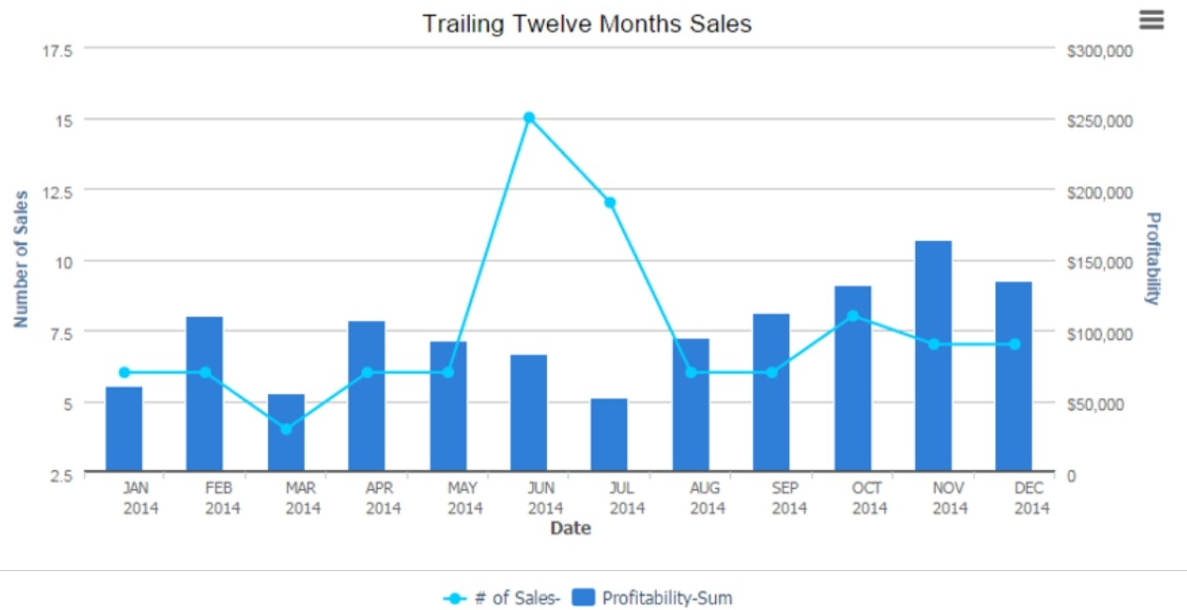
\includegraphics[width=0.85\linewidth]{img/di_trailing_sails.png}\end{center}
\ptesub{范文 Model Answer}
\begin{modelbox}
The following graph gives information about trailing twelve months sales. According to this graph, in January, the value of sales is around six. And in February, that of profitability sum is around eight, which is higher. The highest profitability sum is in November, around eleven. Finally, the lowest one of sales is in March, around four. In conclusion, June has the highest value of sales.
\end{modelbox}
\zh{下图给出的是过去十二个月销售额的信息。根据该图，一月份的销售额数值约为 6；二月份的盈利总额约为 8，数值更高。盈利总额的最高点在十一月，约为 11。最后，销售额的最低点在三月，约为 4。总之，六月的销售额数值最高。}
\ptesub{你的作答（AI 语音识别逐词配色）}
\asrlegend
\begin{asrbox}
\sg{this} \sg{graph} \sy{gives} \sg{information} \sg{about} \sg{training} \sr{twelve} \sy{month} \sy{sale} \sg{and} \sy{the} \sg{ex} \sg{accesses} \sy{data} \sr{and} \sr{the} \sy{y} \sr{axis} \sg{is} \sy{number} \sg{of} \sg{sale} \sg{and} \sg{we} \sg{can} \sg{see} \sy{the} \sy{lowest} \sy{one} \sg{is} \sy{in} \sy{the} \sy{july} \sg{two} \sy{thousand} \sg{and} \sg{forty} \sy{is} \sg{five} \sg{percent} \sg{and} \sg{we} \sg{can} \sg{see} \sy{the} \sg{largest} \sy{a} \sy{number} \sy{of} \sg{skills} \sy{is} \sy{in} \sg{november} \sy{two} \sy{thousand} \sg{and} \sg{forty} \sy{is} \sg{about} \sy{ten} \sg{percent} \sg{and} \sg{we} \sg{can} \sg{see} \sg{the} \sr{perfect} \sy{ibility} \sy{of} \sr{it} \sy{um} \sr{in} \sg{there} \sy{is} \sg{from} \sr{a} \sy{january} \sg{to} \sg{december} \sg{will} \sg{be} \sg{increasing} \sg{so}
\end{asrbox}
\smallskip
{\small\textbf{评分：}内容 \sfull{4.5/5} \quad\textperiodcentered\quad 发音 \sfull{71/90} \quad\textperiodcentered\quad 流利度 \spart{51/90}}\quad{\footnotesize\color{gray}（录音 0:40，用时 01:06）}
\end{qblock}

% ---------------- Q20 ----------------
\begin{qblock}{Q20\quad DI \#692\ \ Vehicle Sales}{描述图 · 总分 \textcolor{cAccent}{\bfseries 63}/90}
\ptesub{配图 Image}
\begin{center}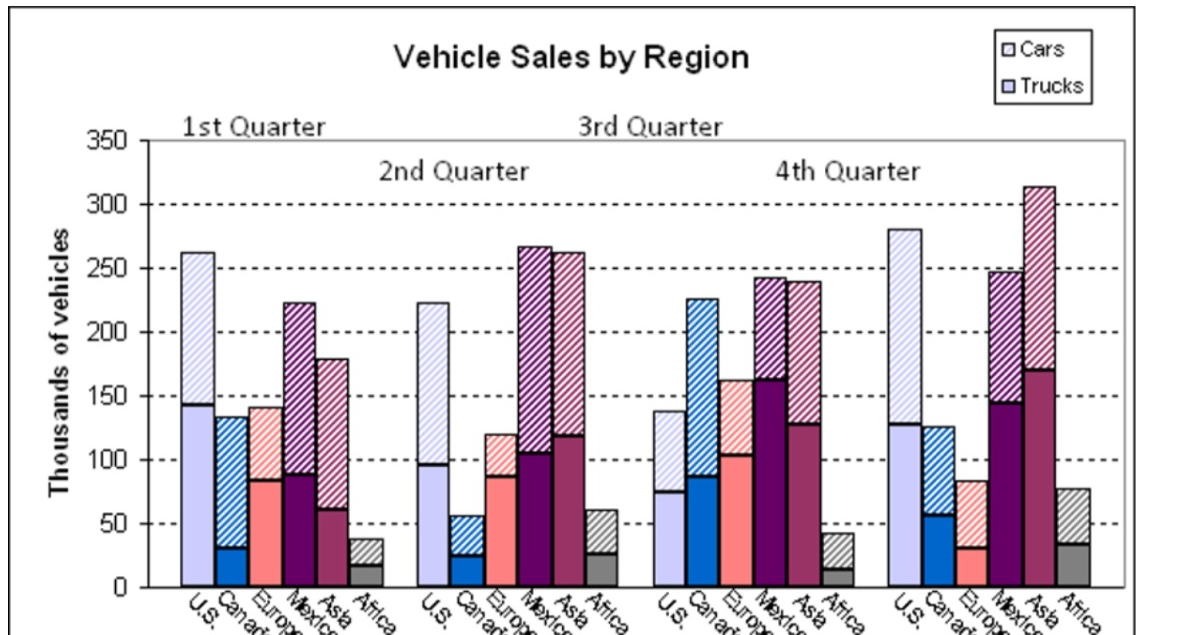
\includegraphics[width=0.85\linewidth]{img/di_vehicle_sales.png}\end{center}
\ptesub{范文 Model Answer}
\begin{modelbox}
The following graph gives information about vehicle sales by region. In the first quarter, the value of US is around two hundred and sixty, and that of Canada is lower, around one hundred and forty. The highest number of Asia is in the fourth quarter, which is three hundred and twenty. Finally, the highest one of Europe is in the third quarter. In conclusion, Africa has the lowest sales.
\end{modelbox}
\zh{下图给出的是各地区车辆销量的信息。第一季度，美国的数值约为 260，而加拿大的数值较低，约为 140。亚洲的最高数值出现在第四季度，为 320。最后，欧洲的最高值出现在第三季度。总之，非洲的销量最低。}
\ptesub{你的作答（AI 语音识别逐词配色）}
\asrlegend
\begin{asrbox}
\sg{we} \sg{can} \sg{see} \sy{the} \sg{following} \sg{graph} \sy{gives} \sg{information} \sg{about} \sg{vehicles} \sy{skill} \sg{by} \sg{religions} \sg{and} \sg{the} \sy{axis} \sy{accesses} \sy{is} \sy{religions} \sg{and} \sy{the} \sy{y} \sg{accesses} \sr{sound} \sy{of} \sy{vehicles} \sg{and} \sg{we} \sg{can} \sg{see} \sg{the} \sg{africa} \sg{is} \sg{always} \sr{the} \sy{smallest} \sg{one} \sg{and} \sy{the} \sy{max} \sr{nicole} \sy{and} \sg{asia} \sg{is} \sg{always} \sg{the} \sy{a} \sg{biggest} \sg{one} \sy{um} \sr{all} \sr{in} \sy{all} \sr{it's} \sg{a} \sy{vehicle} \sg{skill} \sg{by} \sg{regions} \sy{in} \sy{this} \sg{graph}
\end{asrbox}
\smallskip
{\small\textbf{评分：}内容 \sfull{4.5/5} \quad\textperiodcentered\quad 发音 \sfull{72/90} \quad\textperiodcentered\quad 流利度 \spart{56/90}}\quad{\footnotesize\color{gray}（录音 0:40，用时 01:06）}
\end{qblock}

% ---------------- Q21 ----------------
\begin{qblock}{Q21\quad DI \#690\ \ Man at Desk}{描述图 · 总分 \textcolor{cAccent}{\bfseries 59}/90}
\ptesub{配图 Image}
\begin{center}
\includegraphics[width=0.6\linewidth]{img/di_man_at_desk.png}\end{center}
\ptesub{范文 Model Answer}
\begin{modelbox}
The following graph gives information about a man sitting at a desk. In the central area, there is a desk with an open book on it; the color of the book is white. In the right area, it is a laptop with a black keyboard; the color of it is silver. The background has a big screen of a desktop, with a black frame. The weather is sunny. The man is sitting in the chair at the desk. To sum up, the graph tells about a man at the desk.
\end{modelbox}
\zh{下图给出的是一名男子坐在桌前的信息。在中间区域，桌上放着一本打开的书，书的颜色是白色。在右侧区域，是一台带黑色键盘的笔记本电脑，机身颜色是银色。背景中有一个大型台式电脑屏幕，边框是黑色的。天气晴朗，这名男子正坐在桌边的椅子上。总而言之，该图讲述的是一名男子在书桌前的情景。}
\ptesub{你的作答（AI 语音识别逐词配色）}
\asrlegend
\begin{asrbox}
\sg{we} \sg{can} \sg{see} \sg{the} \sy{following} \sy{graph} \sy{gives} \sg{information} \sg{about} \sy{a} \sg{man} \sg{who} \sg{is} \sy{a} \sy{using} \sy{his} \sg{computer} \sy{and} \sy{watching} \sg{his} \sg{book} \sg{we} \sg{can} \sg{see} \sy{the} \sy{man} \sy{is} \sy{where} \sr{a} \sy{two} \sr{to} \sy{a} \sy{t-shirt} \sg{and} \sy{on} \sy{the} \sg{central} \sg{of} \sg{the} \sg{graph} \sy{is} \sr{a} \sg{book} \sg{and} \sr{on} \sy{the} \sy{left} \sy{are} \sr{you} \sy{off} \sy{the} \sy{graph} \sy{we} \sg{can} \sy{see} \sy{three} \sg{computers} \sy{in} \sg{it} \sr{i'm} \sr{all} \sr{in} \sy{all} \sr{it's} \sy{a} \sy{photo} \sy{about} \sr{a} \sg{man} \sg{who} \sg{is} \sg{watching} \sg{his} \sy{books} \sy{and} \sg{watching} \sg{his} \sg{computer}
\end{asrbox}
\smallskip
{\small\textbf{评分：}内容 \sfull{4.3/5} \quad\textperiodcentered\quad 发音 \sfull{68/90} \quad\textperiodcentered\quad 流利度 \spart{58/90}}\quad{\footnotesize\color{gray}（录音 0:40，用时 01:06）}
\end{qblock}

\ptetask{情景应答}{Respond to a Situation · RTS　Q22--24（评分含恰当性）}
% ---------------- Q22 ----------------
\begin{qblock}{Q22\quad RTS (C) \#29\ \ Birthday Activity}{情景应答 · 总分 \textcolor{cAccent}{\bfseries 40}/90}
\ptesub{情景 Situation}
\begin{promptbox}
You're organizing a team outing to celebrate a colleague's birthday-Dave, and everyone's suggesting different activities. However, you realize that some options might not be suitable due to varying preferences and physical abilities. You need to gently guide the discussion towards inclusive activities that everyone can enjoy regardless of their interests or limitations. What would you say to your colleagues?
\end{promptbox}
\zh{你正在组织一次团队出游来庆祝同事戴夫（Dave）的生日，大家都在建议不同的活动。然而你意识到，由于每个人的偏好和身体条件不同，有些方案可能并不合适。你需要温和地把讨论引向那种不论兴趣或身体限制、人人都能享受的包容性活动。你会对同事们说什么？}
\ptesub{参考答案 Model Answer}
\begin{modelbox}
Hey team, I'm thrilled about planning our outing for Dave's birthday! Let's consider activities that everyone can participate in comfortably. How about we go for a picnic in the park or have a game night at someone's place? These options cater to various interests and physical abilities, ensuring everyone has a great time. Let's focus on creating inclusive and enjoyable memories together!
\end{modelbox}
\zh{嘿，团队们，我很期待为戴夫的生日筹划这次出游！让我们考虑那些每个人都能舒适参与的活动。不如我们去公园野餐，或者在某人家里搞一个游戏之夜？这些选择能兼顾各种兴趣和身体条件，确保每个人都玩得开心。让我们专注于一起创造包容而愉快的回忆吧！}
\ptesub{你的作答（AI 语音识别逐词配色）}
\asrlegend
\begin{asrbox}
\sy{hi} \sg{everyone} \sy{welcome} \sg{to} \sg{this} \sg{celebrating} \sg{'s} \sg{and} \sy{i} \sg{notice} \sg{that} \sy{a} \sg{everyone} \sy{suggest} \sg{different} \sg{activities} \sg{but} \sg{i} \sy{realize} \sg{that} \sg{some} \sg{options} \sg{might} \sg{not} \sg{be} \sg{suitable} \sg{due} \sg{to} \sy{very} \sy{preference} \sg{and} \sg{cycle} \sg{abilities} \sg{so} \sg{i} \sy{think} \sr{that's} \sr{a} \sy{can} \sg{join} \sg{the} \sr{a} \sr{a} \sy{discussion} \sr{is} \sy{of} \sy{their} \sg{interest} \sy{and} \sg{limitations} \sy{let's} \sg{have} \sg{a} \sg{good} \sg{time}
\end{asrbox}
\smallskip
{\small\textbf{评分：}恰当性 \spart{56/90} \quad\textperiodcentered\quad 发音 \spart{32/90} \quad\textperiodcentered\quad 流利度 \spart{40/90}}\quad{\footnotesize\color{gray}（录音 0:34，用时 01:29）}
\end{qblock}

% ---------------- Q23 ----------------
\begin{qblock}{Q23\quad RTS (C) \#30\ \ Group Presentation}{情景应答 · 总分 \textcolor{cAccent}{\bfseries 46}/90}
\ptesub{情景 Situation}
\begin{promptbox}
You're preparing for a group presentation, and your team members suggest incorporating complex charts and graphs into the slides. However, you realize that these visuals might confuse the audience and distract from the main points. You need to gently steer the discussion towards simpler and clearer visuals that enhance understanding. What would you say to your team members?
\end{promptbox}
\zh{你正在准备一次小组演示，团队成员建议在幻灯片中加入复杂的图表和图形。然而你意识到，这些视觉元素可能会让听众感到困惑，并分散他们对要点的注意力。你需要温和地把讨论引向更简单、更清晰、有助于理解的视觉呈现方式。你会对团队成员说什么？}
\ptesub{参考答案 Model Answer}
\begin{modelbox}
Hey guys, I appreciate the suggestion for the presentation slides. However, let's aim for simpler visuals to ensure our audience grasps the main points easily. How about we use straightforward charts and diagrams that highlight key information without overwhelming them? This way, we can enhance understanding and keep everyone engaged throughout the presentation. Let's prioritize clarity and effectiveness in our visuals.
\end{modelbox}
\zh{嘿，大家好，谢谢你们对演示幻灯片提出的建议。不过，让我们力求更简洁的视觉呈现，以确保听众能轻松抓住要点。不如我们使用简单明了的图表和示意图，突出关键信息又不让人应接不暇？这样一来，我们就能增进理解，让大家在整个演示过程中都保持专注。让我们把清晰和效果放在视觉设计的首位吧。}
\ptesub{你的作答（AI 语音识别逐词配色）}
\asrlegend
\begin{asrbox}
\sg{hey} \sg{guys} \sy{welcome} \sg{to} \sg{this} \sg{group} \sy{presentation} \sg{and} \sg{i} \sg{have} \sy{notice} \sy{you} \sg{are} \sg{suggesting} \sg{incorporating} \sy{complex} \sr{charts} \sy{and} \sg{graphs} \sg{into} \sg{the} \sg{slides} \sg{however} \sy{i} \sg{notice} \sy{that} \sy{this} \sg{visual} \sy{might} \sg{confuse} \sg{a} \sg{audience} \sg{and} \sy{distract} \sg{from} \sg{the} \sy{main} \sg{points} \sy{i} \sy{think} \sy{it's} \sg{make} \sg{this} \sy{discussions} \sy{over} \sg{the} \sg{simpler} \sy{and} \sg{clear} \sg{visual} \sg{than} \sy{in-house} \sg{understanding} \sg{let's} \sg{go}
\end{asrbox}
\smallskip
{\small\textbf{评分：}恰当性 \sfull{62/90} \quad\textperiodcentered\quad 发音 \spart{41/90} \quad\textperiodcentered\quad 流利度 \spart{43/90}}\quad{\footnotesize\color{gray}（录音 0:34，用时 01:28）}
\end{qblock}

% ---------------- Q24 ----------------
\begin{qblock}{Q24\quad RTS (C) \#31\ \ A Charity Event}{情景应答 · 总分 \textcolor{cAccent}{\bfseries 25}/90}
\ptesub{情景 Situation}
\begin{promptbox}
You're coordinating a charity event for your company, and your team proposes hosting a silent auction to raise funds. However, you realize that organizing the auction might require more resources and time than anticipated. You need to gently guide the discussion towards simpler fundraising ideas. What would you say to your team?
\end{promptbox}
\zh{你正在为公司统筹一场慈善活动，团队提议举办一场无声拍卖来筹款。然而你意识到，筹办这场拍卖可能需要比预想更多的资源和时间。你需要温和地把讨论引向更简单的筹款方案。你会对团队说什么？}
\ptesub{参考答案 Model Answer}
\begin{modelbox}
Hey team, I love the idea of a silent auction for our charity event, but let's consider simpler alternatives that are equally effective. How about organizing a bake sale or a raffle instead? These options require less time and resources to set up but still have the potential to raise significant funds for our cause. Let's brainstorm some creative ideas that align with our goals and resources.
\end{modelbox}
\zh{嘿，团队们，我很喜欢为我们的慈善活动办一场无声拍卖的想法，不过让我们考虑一些同样有效但更简单的替代方案吧。不如我们改为组织一场义卖蛋糕或抽奖活动？这些方案花费的时间和资源更少，却仍有可能为我们的事业筹到可观的善款。让我们一起头脑风暴一些既有创意、又契合我们目标和资源的点子吧。}
\ptesub{你的作答（AI 语音识别逐词配色）}
\asrlegend
\begin{asrbox}
\sg{hey} \sg{guys} \sy{thank} \sg{you} \sg{to} \sg{help} \sg{me} \sg{to} \sg{call} \sy{coordinate} \sy{or} \sy{clarity} \sg{events} \sy{of} \sg{our} \sg{company} \sg{but} \sg{i} \sg{have} \sg{realized} \sg{that} \sy{the} \sg{organizing} \sg{and} \sy{the} \sy{active} \sy{might} \sg{require} \sg{more} \sg{resources} \sg{and} \sg{the} \sy{time} \sr{than} \sy{anticipated} \sy{so} \sg{let's} \sg{make} \sg{the} \sg{discussion} \sr{towards} \sg{simpler} \sy{fundraise} \sg{ideas} \sy{i} \sg{think} \sg{that} \sy{we} \sg{can} \sg{make} \sy{our} \sg{company} \sy{a} \sy{good} \sr{i'm} \sy{more} \sy{and} \sy{more} \sg{healthy} \sy{um} \sy{so} \sg{let's} \sg{go} \sr{okay} \sr{okay}
\end{asrbox}
\smallskip
{\small\textbf{评分：}恰当性 \spart{41/90} \quad\textperiodcentered\quad 发音 \szero{18/90} \quad\textperiodcentered\quad 流利度 \spart{24/90}}\quad{\footnotesize\color{gray}（录音 0:38，用时 01:30）}
\end{qblock}

\ptetask{简短回答}{Answer Short Question · ASQ　Q25--30（单题 0/1）}
\begin{notebox}
{\footnotesize\color{gray}ASQ 考查听问答词，单题 0/1。你的录音不收；下表为题目、中文翻译与参考答案（绿）。}
\smallskip\par
\textbf{Q25\quad ASQ \#1391}\quad{\footnotesize\color{gray}（用时 00:16，得分 \szero{0/1}）}\\
What do we call the fabric that covers the floor of an apartment?\\
\zh{我们把覆盖公寓地板的织物叫做什么？}\\
参考答案：{\color{cFix}\textbf{Carpet / carpets}}（地毯）
\par\smallskip
\textbf{Q26\quad ASQ \#1390}\quad{\footnotesize\color{gray}（用时 00:18，得分 \szero{0/1}）}\\
What do we call the room that is below the level of the ground?\\
\zh{我们把低于地面水平的房间叫做什么？}\\
参考答案：{\color{cFix}\textbf{Basement / cellar}}（地下室 / 地窖）
\par\smallskip
\textbf{Q27\quad ASQ \#1385}\quad{\footnotesize\color{gray}（用时 00:19，得分 \szero{0/1}）}\\
What do we usually call a person who is receiving medical treatment in a hospital?\\
\zh{我们通常把在医院接受治疗的人叫做什么？}\\
参考答案：{\color{cFix}\textbf{Patient / patients}}（病人）
\par\smallskip
\textbf{Q28\quad ASQ \#1384}\quad{\footnotesize\color{gray}（用时 00:18，得分 \szero{0/1}）}\\
Which piece of equipment is used to control the direction of ships?\\
\zh{哪种设备是用来控制船只方向的？}\\
参考答案：{\color{cFix}\textbf{Rudder / rudders}}（舵）
\par\smallskip
\textbf{Q29\quad ASQ \#1382}\quad{\footnotesize\color{gray}（用时 00:18，得分 \szero{0/1}）}\\
Which one is a psychologist good at, surgery or therapy?\\
\zh{心理学家更擅长哪一项，外科手术还是心理治疗？}\\
参考答案：{\color{cFix}\textbf{Therapy}}（心理治疗）
\par\smallskip
\textbf{Q30\quad ASQ \#1381}\quad{\footnotesize\color{gray}（用时 00:18，得分 \szero{0/1}）}\\
What do we call the vacation taken by a couple who have just got married?\\
\zh{我们把新婚夫妇度的假叫做什么？}\\
参考答案：{\color{cFix}\textbf{Honeymoon}}（蜜月）
\end{notebox}

\clearpage
% ===== sec_reading_body.tex =====
% ===================== 阅读 Reading =====================
\ptesection{阅读}{Reading · FIB + MCM-R + RO + FIBD\&D + MCS-R}{42}

\vspace{1mm}
{\small\color{gray} 本部分共 \textbf{16 题}：\textbf{FIB 读写填空}（下拉选词）Q1--5、\textbf{MCM-R 多选}Q6--7、\textbf{RO 段落重排}Q8--9、\textbf{FIBD\&D 读填空}（拖词入空）Q10--14、\textbf{MCS-R 单选}Q15--16。
每题保留文章原文、你的作答（空处对错与平台一致：\rok{绿勾}=选对，{\color{cWrong}\ding{55}}\,红叉=选错并给正确答案）、选项/词库（正确项加粗）、你的答案与得分；并为每篇文章附\textbf{中文翻译}。本套阅读总分 \textbf{42 / 90}。}
\vspace{1mm}

{\small\color{gray}\textbf{说明：}本套复盘截图里每个空后面都有一个「？」小图标（点开显示解析气泡），但截图本身只在个别题上恰好停留在展开状态——\textbf{仅 Q13 的解析被完整截了下来}，其余题目的解析气泡未展开，故从略（如需可到平台点「？」或「查看原题」补看）。}
\vspace{2mm}

\newcolumntype{Z}{>{\RaggedRight\arraybackslash}X}

% ---------------- Q1 ----------------
\begin{qblock}{Q1\quad FIB \#384\ \ Starvation}{读写填空 · 评分 \textcolor{cAccent}{\bfseries 3 / 5}}
\ptesub{文章 Passage（含填空作答）}
\begin{promptbox}
Over weeks and months, malnutrition can result in specific diseases, like anemia when people don't get enough iron or beriberi if they don't get adequate thiamine. A \rno{distinctive}{severe} lack of food for a prolonged period --- not enough calories of any sort to keep up with the body's energy needs --- is starvation. The body's reserve resources are \rok{depleted}. The result is substantial weight loss, wasting away of the body's tissues and eventually death. When faced with starvation, the body fights back. The first day without food is a lot like the overnight fast between dinner one night and breakfast the next morning. Energy levels are low but \rno{feed}{pick} up with a morning meal. Within days, faced with nothing to eat, the body begins feeding on itself. Metabolism slows; the body cannot regulate its temperature; kidney function is impaired and the immune system \rok{weakens}. When the body uses its reserves to provide basic energy needs, it can no longer supply necessary nutrients to vital organs and tissues. The heart, lungs, ovaries and testes shrink. Muscles shrink and people feel weak. Body temperature drops and people can feel chilled. People can become \rok{irritable}, and they become difficult to concentrate.
\end{promptbox}
\zh{经过数周乃至数月，营养不良会导致特定疾病，比如缺铁引起的贫血，或缺乏足量硫胺素引起的脚气病。长期严重缺乏食物——任何种类的热量都不足以维持身体能量需求——就是饥饿。此时身体的储备资源被耗尽，结果是体重大幅下降、身体组织逐渐消耗，最终死亡。面对饥饿，身体会做出反抗：不进食的第一天很像晚饭到次日早饭之间的整夜禁食，能量水平较低，但早餐后又能恢复。几天之内，面对无物可食，身体开始"吃自己"：代谢减慢，身体无法调节体温，肾功能受损，免疫系统减弱。当身体动用储备来满足基本能量需求时，就无法再向重要器官和组织供应必需的营养——心脏、肺、卵巢和睾丸都会萎缩，肌肉萎缩、人变得虚弱，体温下降、人会感到发冷。人还可能变得易怒，难以集中注意力。}
\ptesub{选项 Choices（每空 4 选 1，正确项加粗）}
{\small
1.\ \textbf{severe},\ distinguishing,\ proper,\ distinctive\\
2.\ obsoleted,\ \textbf{depleted},\ pelleted,\ deleted\\
3.\ feed,\ come,\ chill,\ \textbf{pick}\\
4.\ deepens,\ deafens,\ \textbf{weakens},\ surpasses\\
5.\ \textbf{irritable},\ commutable,\ indisputable,\ transportable}
\par\smallskip
\textbf{你的答案：}\ {\color{cWrong}distinctive}, depleted, {\color{cWrong}feed}, weakens, irritable\qquad\textbf{本题得分：}\ {\color{cAccent}\bfseries 3 / 5}\quad{\footnotesize\color{gray}（用时 02:28；第 1 空 distinctive→severe、第 3 空 feed→pick）}
\end{qblock}

% ---------------- Q2 ----------------
\begin{qblock}{Q2\quad FIB \#380\ \ Death Sentence}{读写填空 · 评分 \textcolor{cAccent}{\bfseries 2 / 5}}
\ptesub{文章 Passage（含填空作答）}
\begin{promptbox}
You are more likely to be \rok{sentenced} to death if you are a member of a minority group within a state that executes defendants. The death penalty disproportionately affects members of racial, ethnic and religious minorities, as well as those living in poverty. In the US, there's extensive evidence of racial \rno{appearance}{bias} on death row. The race of the victim remains the single most reliable factor in \rok{determining} whether a defendant will be given a death sentence. African American defendants are three times more likely to receive the death penalty than white defendants, where the victims are white. Serious mental health issues are also common in defendants sent to death row. At least one in ten prisoners \rno{persecuted}{executed} in the US between 1977 and 2007 had experienced severe mental health problems that meant they were literally unable to comprehend the crime they were \rno{persuaded}{alleged} to have committed, and unable to understand the terms of their sentence and imminent execution.
\end{promptbox}
\zh{如果你是执行死刑的州里少数群体的一员，你被判死刑的可能性更高。死刑不成比例地影响着种族、族裔和宗教上的少数群体，以及生活在贫困中的人。在美国，有大量证据表明死囚群体中存在种族偏见。受害者的种族仍然是决定被告是否会被判死刑的最可靠单一因素——当受害者是白人时，非裔美国被告被判死刑的可能性是白人被告的三倍。严重的心理健康问题在死囚犯中也很常见：1977年至2007年间，美国至少有十分之一被处决的囚犯曾经历严重的心理健康问题，以至于他们实际上根本无法理解自己被指控所犯下的罪行，也无法理解判决的内容和即将到来的处决。}
\ptesub{选项 Choices（每空 4 选 1，正确项加粗）}
{\small
1.\ penalized,\ blamed,\ complained,\ \textbf{sentenced}\\
2.\ \textbf{bias},\ equality,\ appearance,\ background\\
3.\ \textbf{determining},\ adjoining,\ undermining,\ examining\\
4.\ electrocuted,\ persecuted,\ \textbf{executed},\ captured\\
5.\ \textbf{alleged},\ acclaimed,\ persuaded,\ claimed}
\par\smallskip
\textbf{你的答案：}\ sentenced, {\color{cWrong}appearance}, determining, {\color{cWrong}persecuted, persuaded}\qquad\textbf{本题得分：}\ {\color{cAccent}\bfseries 2 / 5}\quad{\footnotesize\color{gray}（用时 02:13；第 2 空 appearance→bias、第 4 空 persecuted→executed、第 5 空 persuaded→alleged）}
\end{qblock}

% ---------------- Q3 ----------------
\begin{qblock}{Q3\quad FIB \#381\ \ Deception}{读写填空 · 评分 \textcolor{cAccent}{\bfseries 3 / 5}}
\ptesub{文章 Passage（含填空作答）}
\begin{promptbox}
Deception refers to the act of \rok{encouraging} people to believe information that is not true. Lying is a common form of deception, stating something known to be untrue with the intent to deceive. While most people are generally honest, even those who \rok{subscribe} to honesty engage in deception sometimes. Studies show that the average person lies several times a day. Some of those lies are big (`I've never cheated on you!') but more often, they are little white lies (`That dress looks fine') deployed to \rok{avoid} uncomfortable situations or spare someone's feelings. Trust is the bedrock of social life at all levels, from romance and parenting to national government. Deception always \rno{undertakes}{undermines} it. Because truth is so essential to the human enterprise, which relies on a shared view of reality, the default assumption most people have is that others are truthful in their communications and dealings. Most cultures have powerful social \rno{ejections}{sanctions} against lying.
\end{promptbox}
\zh{欺骗是指让人们相信不真实信息的行为。撒谎是欺骗的一种常见形式，即明知某事不实、却出于欺骗意图而陈述它。虽然大多数人总体上是诚实的，但即便是信奉诚实的人有时也会进行欺骗。研究显示，普通人平均每天会撒谎好几次。其中有些谎言很大("我从没有出轨过！")，但更多时候是善意的小谎言("这条裙子看起来挺好")，用来避免尴尬处境或顾及他人感受。信任是社会生活各个层面的基石，从恋爱、为人父母到国家治理概莫能外。欺骗总是会破坏信任。因为真相对依赖共享现实观的人类社会而言至关重要，大多数人默认的假设是：他人在交流与交往中是诚实的。大多数文化都有强有力的社会性制裁来对抗撒谎。}
\ptesub{选项 Choices（每空 4 选 1，正确项加粗）}
{\small
1.\ discouraging,\ forbidding,\ detecting,\ \textbf{encouraging}\\
2.\ describe,\ prescribe,\ inscribe,\ \textbf{subscribe}\\
3.\ contest,\ illuminate,\ disguise,\ \textbf{avoid}\\
4.\ \textbf{undermines},\ underscores,\ undertakes,\ underwrites\\
5.\ ejections,\ \textbf{sanctions},\ fractions,\ inductions}
\par\smallskip
\textbf{你的答案：}\ encouraging, subscribe, avoid, {\color{cWrong}undertakes, ejections}\qquad\textbf{本题得分：}\ {\color{cAccent}\bfseries 3 / 5}\quad{\footnotesize\color{gray}（用时 02:06；第 4 空 undertakes→undermines、第 5 空 ejections→sanctions）}
\end{qblock}

% ---------------- Q4 ----------------
\begin{qblock}{Q4\quad FIB \#373\ \ Information Revolution}{读写填空 · 评分 \textcolor{cAccent}{\bfseries 1 / 5}}
\ptesub{文章 Passage（含填空作答）}
\begin{promptbox}
Some have begun to call it the Information Revolution. Technological changes brought dramatic new \rok{options} to Americans living in the 1990s. From the beginning of the decade until the end, new forms of entertainment, commerce, research, work, and communication became commonplace in the United States. The \rno{unremitting}{driving} force behind much of this change was an innovation popularly known as the Internet. Personal computers had become widespread by the end of the 1980s. Through a device called a modem, individual users could link their computer to a \rno{volume}{wealth} of information using conventional phone lines. What lay beyond the individual computer was a vast domain of information known as cyberspace. Upon its \rno{relief}{release} in 1983 the Apple ``Lisa'' computer was supposed to revolutionize personal computing. But interest in ``Lisa'' was minimal due to its nearly \$10,000 price tag and the introduction of the much more \rno{advanced}{affordable} ``Macintosh'' a year later.
\end{promptbox}
\zh{有人已经开始称之为"信息革命"。技术变革为20世纪90年代的美国人带来了戏剧性的全新选择。从这十年之初到末尾，新形式的娱乐、商业、研究、工作和通讯在美国变得司空见惯。推动这一变化的主要力量，是一项被普遍称为"互联网"的创新。到20世纪80年代末，个人电脑已经普及。通过一种叫做调制解调器的设备，个人用户可以借助传统电话线将自己的电脑连接到海量的信息资源上。个人电脑之外，还存在一个被称为"网络空间"的广阔信息领域。1983年发布的苹果"Lisa"电脑本应彻底革新个人计算，但由于其近一万美元的高价，加上一年后推出的价格更加亲民的"Macintosh"，人们对"Lisa"的兴趣微乎其微。}
\ptesub{选项 Choices（每空 4 选 1，正确项加粗）}
{\small
1.\ challenges,\ puzzles,\ \textbf{options},\ confusion\\
2.\ unremitting,\ uninspiring,\ \textbf{driving},\ insinuating\\
3.\ magnitude,\ bulk,\ \textbf{wealth},\ volume\\
4.\ relief,\ \textbf{release},\ publication,\ emission\\
5.\ convenient,\ \textbf{affordable},\ advanced,\ formidable}
\par\smallskip
\textbf{你的答案：}\ options, {\color{cWrong}unremitting, volume, relief, advanced}\qquad\textbf{本题得分：}\ {\color{cAccent}\bfseries 1 / 5}\quad{\footnotesize\color{gray}（用时 02:53；仅第 1 空 options 正确，其余四空全错）}
\end{qblock}

% ---------------- Q5 ----------------
\begin{qblock}{Q5\quad FIB \#372\ \ Dentistry}{读写填空 · 评分 \textcolor{cAccent}{\bfseries 2 / 4}}
\ptesub{文章 Passage（含填空作答）}
\begin{promptbox}
Dentistry is a profession \rno{dealt}{concerned} with the prevention and treatment of oral disease. Dentistry also encompasses the treatment and correction of malformation of the jaws, misalignment of the teeth, and birth anomalies of the oral cavity such as cleft palate. Dentistry, in some form, has been \rok{practiced} since ancient times. For example, Egyptian skulls dating from 2900 to 2750 BCE contain evidence of small holes in the jaw in the vicinity of a tooth's roots. Such holes are believed to have been \rno{laminated}{drilled} to drain abscesses. In addition, accounts of dental treatment appear in Egyptian scrolls dating from 1500 BCE. It is thought that the Egyptians practiced oral surgery perhaps as early as 2500 BCE, although evidence for this is minimal. An early attempt at tooth \rok{replacement} dates to Phoenicia (modern Lebanon) around 600 BCE, where missing teeth were replaced with animal teeth and were bound into place with cord.
\end{promptbox}
\zh{牙科是一门致力于预防和治疗口腔疾病的专业。牙科还涵盖了对颌骨畸形、牙齿错位以及诸如唇腭裂等口腔先天异常的治疗与矫正。某种形式的牙科诊疗自古以来就已存在：例如，公元前2900年至2750年的埃及头骨上有证据显示，牙根附近的颌骨上有小孔，人们认为这些小孔是被钻开以引流脓肿的。此外，公元前1500年的埃及卷轴中也记载了牙科治疗的内容。据推测，埃及人也许早在公元前2500年就已经进行口腔手术，尽管这方面的证据很少。最早尝试补牙的记录可追溯到约公元前600年的腓尼基（今黎巴嫩），当时缺失的牙齿会用动物牙齿替代，并用绳子绑扎固定。}
\ptesub{选项 Choices（每空 4 选 1，正确项加粗）}
{\small
1.\ agreed,\ dealt,\ \textbf{concerned},\ taken\\
2.\ criticized,\ replaced,\ \textbf{practiced},\ abandoned\\
3.\ fluctuated,\ laminated,\ \textbf{drilled},\ sealed\\
4.\ reparation,\ sacrament,\ restitution,\ \textbf{replacement}}
\par\smallskip
\textbf{你的答案：}\ {\color{cWrong}dealt}, practiced, {\color{cWrong}laminated}, replacement\qquad\textbf{本题得分：}\ {\color{cAccent}\bfseries 2 / 4}\quad{\footnotesize\color{gray}（用时 01:38；第 1 空 dealt→concerned、第 3 空 laminated→drilled）}
\end{qblock}

% ---------------- Q6 ----------------
\begin{qblock}{Q6\quad MCM-R \#118\ \ Taste Sensitivity}{多选 · 评分 \textcolor{cAccent}{\bfseries 1 / 2}}
\ptesub{文章 Passage}
\begin{promptbox}
What you eat influences your taste for what you might want to eat next. So claims a University of California, Riverside, study performed on fruit flies. The study offers a better understanding of neurophysiological plasticity of the taste system in flies. To maintain ideal health, animals require a balanced diet with optimum amounts of different nutrients. Macronutrients like carbohydrates and proteins are essential; indeed, an unbalanced intake of these nutrients can be detrimental to health. Flies require macronutrients such as sugars and amino acids for survival. They use the gustatory system, the sensory system responsible for the perception of taste, to sense these nutrients and begin feeding.

In their experiments in the lab, the researchers Anindya Ganguly and Manali Dey, led by Anupama Dahanukar, fed adult flies different diets: a balanced diet, a sugar-reduced and protein-enriched diet, and a sugar-enriched and protein-depleted diet. They ensured that all three diets were similar in total calorie content and tested the flies daily for a week to examine modifications in their food choice and taste sensitivity. The researchers report that diet affects dopamine and insulin signaling in the brain, which, in turn, affects the flies' peripheral sensory response, which is comprised of neurons directly involved in detecting external stimuli. This response then influences what the flies eat next.
\end{promptbox}
\zh{你所吃的食物会影响你接下来想吃什么口味的东西——加州大学河滨分校一项针对果蝇的研究如是说。该研究让我们更好地理解了果蝇味觉系统的神经生理可塑性。为保持理想的健康状态，动物需要摄入均衡的饮食，各种营养素的量都要恰到好处。碳水化合物和蛋白质这类宏量营养素是必需的；事实上，这些营养素摄入不均衡会损害健康。果蝇的生存需要糖和氨基酸等宏量营养素，它们利用负责感知味道的感觉系统——味觉系统——来感知这些营养素并开始进食。在实验室实验中，由 Anupama Dahanukar 带领的研究人员 Anindya Ganguly 和 Manali Dey 给成年果蝇喂食了三种不同的饮食：均衡饮食、低糖高蛋白饮食，以及高糖低蛋白饮食。他们确保这三种饮食的总热量相近，并每天对果蝇进行为期一周的测试，以观察它们食物选择和味觉敏感度的变化。研究人员报告称，饮食会影响大脑中多巴胺和胰岛素的信号传导，进而影响果蝇的外周感觉反应——该反应由直接参与探测外部刺激的神经元构成。这种反应接下来又会影响果蝇下一步吃什么。}
\ptesub{题目 Question}
\begin{notebox}Which of the following statements about the study are true?\end{notebox}
\ptesub{选项 Choices（正确项绿色加粗）}
{\small
A) What you eat has little to do with what you want to eat next.\\
B) An unbalanced intake of macronutrients such as carbohydrates and protein is essential.\\
{\color{cFix}\textbf{C) The fly senses macronutrients through its taste system.}}\\
D) In the experiment, the researchers made sure the total calories in all three diets were the same.\\
E) The researchers tested the flies every two days for a week.\\
{\color{cFix}\textbf{F) Dopamine in the brain is closely related to diet.}}}
\par\smallskip
\textbf{正确答案}\ \textcolor{cFix}{\bfseries C, F}\qquad\textbf{你的答案}\ {\color{cWrong}\bfseries F}\qquad\textbf{本题得分：}\ {\color{cAccent}\bfseries 1 / 2}\quad{\footnotesize\color{gray}（用时 00:37；只选了 F，漏选 C）}
\end{qblock}

% ---------------- Q7 ----------------
\begin{qblock}{Q7\quad MCM-R \#114\ \ Persistent Back Pain}{多选 · 评分 \textcolor{cAccent}{\bfseries 0 / 2}}
\ptesub{文章 Passage}
\begin{promptbox}
People with persistent back pain or persistent headaches are twice as likely to suffer from both disorders, a new study from the University of Warwick has revealed.

The results, published in the Journal of Headache and Pain, suggest an association between the two types of pain that could point to a shared treatment for both.

The researchers from Warwick Medical School who are funded by the National Institute for Health Research (NIHR) led a systematic review of fourteen studies with a total of 460,195 participants that attempt to quantify the association between persistent headaches and persistent low back pain. They found an association between having persistent low back pain and having persistent (chronic) headaches, with patients experiencing one typically being twice as likely to experience the other compared to people without either headaches or back pain. The association is also stronger for people affected by migraine.

The researchers focused on people with chronic headache disorders, those who will have had headaches on most days for at least three months, and people with persistent low back pain that experience that pain day after day. These are two very common disorders that are leading causes of disability worldwide. Around one in five people have persistent low back pain and one in 30 have chronic headaches. The researchers estimate that just over one in 100 people (or well over half a million people) in the UK have both.
\end{promptbox}
\zh{华威大学一项新研究显示，患有持续性背痛或持续性头痛的人，同时患上这两种病症的可能性会翻倍。这项发表于《头痛与疼痛期刊》的研究结果，提示这两类疼痛之间存在关联，或可指向二者共同的治疗方法。由英国国家健康研究所（NIHR）资助的华威医学院研究人员，主导了一项系统综述，纳入14项研究、共46万零195名参与者，试图量化持续性头痛与持续性下背痛之间的关联。他们发现，患有持续性下背痛与患有持续性（慢性）头痛之间存在关联：与既无头痛也无背痛的人相比，患有其中一种病症的人患上另一种的可能性通常会翻倍；这种关联在偏头痛患者中更为明显。研究人员聚焦于患有慢性头痛病症的人（即在至少三个月里大多数日子都头痛的人），以及日复一日持续背痛的持续性下背痛患者。这是两种全球范围内导致残疾的主要常见病症：约五分之一的人患有持续性下背痛，三十分之一的人患有慢性头痛。研究人员估计，在英国，略超过百分之一的人（远超五十万人）同时患有这两种病症。}
\ptesub{题目 Question}
\begin{notebox}What are the main findings of the study?\end{notebox}
\ptesub{选项 Choices（正确项绿色加粗）}
{\small
{\color{cFix}\textbf{A) In the UK, one in 100 people have both persistent back pain and persistent headaches.}}\\
{\color{cFix}\textbf{B) There is a link between persistent back pain and persistent headache.}}\\
C) Headaches are the only cause of disability.\\
D) People with persistent back pain or headaches are half as likely to develop either condition.\\
E) The relationship between persistent headache and persistent low back pain is not quantifiable.}
\par\smallskip
\textbf{正确答案}\ \textcolor{cFix}{\bfseries A, B}\qquad\textbf{你的答案}\ {\color{cWrong}\bfseries E}\qquad\textbf{本题得分：}\ {\color{cAccent}\bfseries 0 / 2}\quad{\footnotesize\color{gray}（用时 00:24，全错）}
\end{qblock}

% ---------------- Q8 ----------------
\begin{qblock}{Q8\quad RO \#365\ \ Joint Venture}{段落重排 · 评分 \textcolor{cAccent}{\bfseries 1 / 3}}
\ptesub{乱序段落 Paragraphs}
\begin{promptbox}
\textbf{1)} A joint venture (JV) is a business arrangement in which two or more parties agree to pool their resources for the purpose of accomplishing a specific task.\\
\textbf{2)} In a JV, each of the participants is responsible for profits, losses, and costs associated with it.\\
\textbf{3)} However, the venture is its own entity, separate from the participants' other business interests.\\
\textbf{4)} This task can be a new project or any other business activity.
\end{promptbox}
\zh{（按正确顺序）合资企业（JV）是一种商业安排，其中两方或以上当事方同意集中各自的资源以完成一项特定任务；这项任务可以是一个新项目，也可以是其他任何商业活动。在合资企业中，每一位参与方都要对与之相关的利润、亏损和成本负责；不过，该合资企业本身是一个独立的实体，与参与方各自的其他商业利益相分离。}
\par\smallskip
\textbf{正确顺序}\ \textcolor{cFix}{\bfseries 1 → 4 → 2 → 3}\qquad\textbf{你的顺序}\ {\color{cWrong}\bfseries 1 → 2 → 3 → 4}\qquad\textbf{本题得分：}\ {\color{cAccent}\bfseries 1 / 3}\quad{\footnotesize\color{gray}（用时 00:35）}
\end{qblock}

% ---------------- Q9 ----------------
\begin{qblock}{Q9\quad RO \#369\ \ Mutations}{段落重排 · 评分 \textcolor{cAccent}{\bfseries 3 / 3}}
\ptesub{乱序段落 Paragraphs}
\begin{promptbox}
\textbf{1)} Others offer benefits, some can do both, and the mutation that underlies sickle cell disease is one that can be both good and very bad.\\
\textbf{2)} Our genes serve as an operating manual for cells of the body.\\
\textbf{3)} Genes tell cells what to do and when. But copying errors in those operating manuals - known as mutations - can lead to misspelled instructions that can change how cells operate.\\
\textbf{4)} Scientists now know that some of those mutations can lead to disease.
\end{promptbox}
\zh{（按正确顺序）我们的基因就像是身体细胞的操作手册。基因告诉细胞该做什么、何时做；但这些操作手册中的复制错误——即所谓的突变——可能导致指令出现"拼写错误"，从而改变细胞的运作方式。科学家现在知道，有些突变会导致疾病；另一些突变则带来益处，还有一些两者兼具——镰状细胞病背后的那个突变，就是一个既能带来好处、也能造成严重危害的突变。}
\par\smallskip
\textbf{正确顺序}\ \textcolor{cFix}{\bfseries 2 → 3 → 4 → 1}\qquad\textbf{你的顺序}\ \textcolor{cFix}{\bfseries 2 → 3 → 4 → 1}\qquad\textbf{本题得分：}\ {\color{cAccent}\bfseries 3 / 3}\quad{\footnotesize\color{gray}（用时 00:42，全对）}
\end{qblock}

% ---------------- Q10 ----------------
\begin{qblock}{Q10\quad FIBD\&D \#554\ \ Vegetative Propagation}{读填空（拖词）· 评分 \textcolor{cAccent}{\bfseries 0 / 4}}
\ptesub{文章 Passage（含填空作答）}
\begin{promptbox}
Because vegetative propagation is a form of asexual reproduction, plants produced through this system are genetic clones of a parent plant. One advantage of vegetative propagation is that plants with \rno{artificial}{favorable} traits are repeatedly reproduced. Commercial crop growers can employ \rno{traditional}{artificial} vegetative propagation techniques to ensure advantageous \rno{capabilities}{qualities} in their crops. A major disadvantage, however, of vegetative propagation is that it does not allow for any degree of genetic \rno{qualities}{variation}.
\end{promptbox}
\zh{由于营养繁殖是一种无性繁殖方式，通过这种方式产生的植物是母株的基因克隆体。营养繁殖的一个优点是，具有优良性状的植物可以被反复复制。商业作物种植者可以采用人工营养繁殖技术，来确保作物具备优良的性状。然而，营养繁殖的一个主要缺点是它完全不允许任何程度的基因变异。}
\ptesub{词库 Word Bank（拖词入空，正确答案加粗）}
{\small 1) \textbf{variation}\quad 2) \textbf{favorable}\quad 3) \textbf{artificial}\quad 4) capabilities\quad 5) diversification\quad 6) \textbf{qualities}\quad 7) traditional}
\par\smallskip
\textbf{你的答案：}\ {\color{cWrong}artificial, traditional, capabilities, qualities}\qquad\textbf{本题得分：}\ {\color{cAccent}\bfseries 0 / 4}\quad{\footnotesize\color{gray}（用时 02:18；四空全错，正确为 favorable / artificial / qualities / variation）}
\end{qblock}

% ---------------- Q11 ----------------
\begin{qblock}{Q11\quad FIBD\&D \#555\ \ Push-pull Factors}{读填空（拖词）· 评分 \textcolor{cAccent}{\bfseries 3 / 4}}
\ptesub{文章 Passage（含填空作答）}
\begin{promptbox}
In geographical terms, the push-pull factors drive people away from a place and \rok{draw} people to a new location. They help \rno{drag}{determine} migration of particular populations from one land to another. Push factors are often \rok{forceful}, demanding that a certain person or group of people leave one country for another. Pull factors, on the other hand, are often the positive policies that encourage people to \rok{immigrate} in order to seek a better life.
\end{promptbox}
\zh{在地理学意义上，推拉因素把人从一个地方推开、又把人吸引到一个新的地方。它们有助于决定特定人群从一片土地迁往另一片土地的迁移情况。推力因素往往带有强制性，迫使某个人或某群人离开一个国家前往另一个国家；而拉力因素则往往是那些鼓励人们为了寻求更好生活而移民的积极政策。}
\ptesub{词库 Word Bank（拖词入空，正确答案加粗）}
{\small 1) \textbf{immigrate}\quad 2) \textbf{forceful}\quad 3) drag\quad 4) \textbf{draw}\quad 5) \textbf{determine}\quad 6) formidable\quad 7) shift}
\par\smallskip
\textbf{你的答案：}\ draw, {\color{cWrong}drag}, forceful, immigrate\qquad\textbf{本题得分：}\ {\color{cAccent}\bfseries 3 / 4}\quad{\footnotesize\color{gray}（用时 01:43；第 2 空 drag→determine）}
\end{qblock}

% ---------------- Q12 ----------------
\begin{qblock}{Q12\quad FIBD\&D \#561\ \ India}{读填空（拖词）· 评分 \textcolor{cAccent}{\bfseries 1 / 4}}
\ptesub{文章 Passage（含填空作答）}
\begin{promptbox}
India's movie history began in 1896 when the Lumière brothers wanted to \rok{demonstrate} the art of cinema in Mumbai. Today, the films are known for their \rno{（未填）}{elaborate} singing and dancing. Indian dance, music and theater traditions \rno{drive}{span} back more than 2,000 years. The major classical dance traditions \rno{elaborate}{draw} on themes from mythology and literature and have rigid presentation rules.
\end{promptbox}
\zh{印度的电影历史始于1896年，卢米埃尔兄弟当时想在孟买展示电影这门艺术。如今，印度电影以其精心编排的歌舞著称。印度的舞蹈、音乐和戏剧传统可以追溯到2000多年前。主要的古典舞蹈传统取材于神话和文学主题，并有着严格的表演规范。}
\ptesub{词库 Word Bank（拖词入空，正确答案加粗）}
{\small 1) detailed\quad 2) \textbf{demonstrate}\quad 3) \textbf{draw}\quad 4) \textbf{span}\quad 5) drive\quad 6) \textbf{elaborate}\quad 7) appraise}
\par\smallskip
\textbf{你的答案：}\ demonstrate, {\color{cWrong}（第 2 空未作答）}, {\color{cWrong}drive, elaborate}\qquad\textbf{本题得分：}\ {\color{cAccent}\bfseries 1 / 4}\quad{\footnotesize\color{gray}（用时 02:20；第 2 空未填（应为 elaborate）、第 3 空 drive→span、第 4 空 elaborate→draw）}
\end{qblock}

% ---------------- Q13 ----------------
\begin{qblock}{Q13\quad FIBD\&D \#102\ \ Volcanoes}{读填空（拖词）· 评分 \textcolor{cAccent}{\bfseries 2 / 4}}
\ptesub{文章 Passage（含填空作答）}
\begin{promptbox}
Volcanoes blast more than 100 million tons of carbon dioxide into the atmosphere every year but the gas is usually \rok{harmless}. When a volcano erupts, carbon dioxide spreads out into the atmosphere and isn't \rok{concentrated} in one spot. But sometimes the gas gets trapped \rno{atmosphere}{underground} under enormous pressure. If it escapes to the surface in a dense \rno{underground}{cloud}, it can push out oxygen-rich air and become deadly.
\end{promptbox}
\zh{火山每年向大气层喷发超过一亿吨的二氧化碳，但这种气体通常是无害的。火山喷发时，二氧化碳会扩散到大气中，不会聚集在一个地点。但有时气体会在巨大的压力下被困在地下；如果它以浓密的云雾形式逃逸到地表，就会把富含氧气的空气挤走，从而变得致命。}
\ptesub{词库 Word Bank（拖词入空，正确答案加粗）}
{\small 1) \textbf{cloud}\quad 2) \textbf{concentrated}\quad 3) dangerous\quad 4) \textbf{harmless}\quad 5) \textbf{underground}\quad 6) air\quad 7) atmosphere\quad 8) collected\quad 9) over}
\ptesub{解析 Explanation（本套仅本题截图恰好展开了解析气泡）}
\begin{notebox}\footnotesize
\textbf{1.\ harmless}\quad 位于动词 is 后，选择形容词，可选的单词有 dangerous(危险的)、harmless(无害的)、harmful(有伤害的)；根据原文 "Volcanoes blast more than 100 million tons of carbon dioxide into the atmosphere every year but the gas is usually \_\_\_"，but 表示前后内容意思对立——前面说大量气体喷发，与之相反的是这些气体对我们没有伤害，故选 harmless。这里说的是：火山每年向大气喷发超过1亿吨的二氧化碳，但气体通常是无害的。【解题思路：主系表结构；转折关系；单句理解】\par\smallskip
\textbf{2.\ concentrated}\quad 位于 isn't 后，且主语为 carbon dioxide，可选择 v-ed 形式构成被动结构也可选择名词或形容词，可选的单词有 cloud(云)、concentrated(积聚)、dangerous(危险)、underground(在地下的)、aimed(瞄准)、air(空气)、harmful(有害的)、atmosphere(大气)、collected(收集)、fact(事实)。根据原文 "When a volcano erupts, carbon dioxide spreads out into the atmosphere and isn't \_\_\_ in one spot"，这里说二氧化碳进入大气层，在一个地点不会发生什么，代入选项，气体不会"聚集"在一个地方，最符合语意。【解题思路：被动语态；近义词辨析；单句理解】\par\smallskip
\textbf{3.\ underground}\quad 该空所在句主干："But sometimes the gas gets trapped \_\_\_ ..."，主干部分完整，因此选择副词作为修饰，可选择的单词有 underground(在地下)、over(倒下、翻转、穿过)。根据原文 "But sometimes the gas gets trapped \_\_\_ under enormous pressure"，由于二氧化碳在巨大的压力下，那应该是在地表下，而不是在水下承受巨大压力，因此选择 underground。这里说的是：但有时气体在巨大的压力下被困在地下。【解题思路：副词做状语；单句理解】\par\smallskip
\textbf{4.\ cloud}\quad 位于形容词 dense 后，选择名词，可选择的单词有 cloud(云)、air(空气)、atmosphere(大气)、collection(收集)、fact(事实)。根据原文 "If it escapes to the surface in a dense \_\_\_, it can push out oxygen-rich air and become deadly"，根据前面的冠词 a 判断，air 和 atmosphere 是不可数的，而 collection 又说不通，因此选择 cloud。这里说的是：如果它以浓稠云雾的形态逃逸出地表，就会排挤富含氧气的空气，从而变得致命。【解题思路：形容词+名词结构；单句理解】
\end{notebox}
\par\smallskip
\textbf{你的答案：}\ harmless, concentrated, {\color{cWrong}atmosphere, underground}\qquad\textbf{本题得分：}\ {\color{cAccent}\bfseries 2 / 4}\quad{\footnotesize\color{gray}（用时 03:18；第 3 空 atmosphere→underground、第 4 空 underground→cloud）}
\end{qblock}

% ---------------- Q14 ----------------
\begin{qblock}{Q14\quad FIBD\&D \#556\ \ Tiger Sharks}{读填空（拖词）· 评分 \textcolor{cAccent}{\bfseries 0 / 4}}
\ptesub{文章 Passage（含填空作答）}
\begin{promptbox}
The tiger shark is named for the dark, vertical stripes on either side of its body, which are reminiscent of a tiger's \rno{feature}{markings}. These stripes actually \rno{transplant}{fade} as the tiger shark ages, so they can't be used as an identifying \rno{markings}{feature} of every individual. Young tiger sharks have dark blotches or spots, which eventually \rno{fade}{merge} into stripes. For this reason, the species is sometimes known as the leopard shark or the spotted shark.
\end{promptbox}
\zh{虎鲨之所以得名，是因为它身体两侧有着让人联想到老虎斑纹的深色竖条纹。这些条纹实际上会随着虎鲨年龄的增长而褪色，因此不能作为辨识每一个个体的特征。幼年虎鲨身上有深色的斑块或斑点，这些斑点最终会融合成条纹。因此，这个物种有时也被称为豹纹鲨或斑点鲨。}
\ptesub{词库 Word Bank（拖词入空，正确答案加粗）}
{\small 1) transplant\quad 2) \textbf{merge}\quad 3) function\quad 4) \textbf{feature}\quad 5) \textbf{markings}\quad 6) \textbf{fade}\quad 7) detection}
\par\smallskip
\textbf{你的答案：}\ {\color{cWrong}feature, transplant, markings, fade}\qquad\textbf{本题得分：}\ {\color{cAccent}\bfseries 0 / 4}\quad{\footnotesize\color{gray}（用时 01:50；四空全错，正好错位一个：正确为 markings / fade / feature / merge）}
\end{qblock}

% ---------------- Q15 ----------------
\begin{qblock}{Q15\quad MCS-R \#160\ \ Walking Stamina}{单选 · 评分 \textcolor{cAccent}{\bfseries 1 / 1}}
\ptesub{文章 Passage}
\begin{promptbox}
If you've decided you want to improve your fitness, walking is a good choice. It's free, simple, and adaptable to your schedule. If you've been relatively sedentary, you might find that you can't walk very far at first without getting sore or out-of-breath. You just have to keep at it! If you try to walk a little further every day, you'll find that your walking stamina gradually improves. If you don't have the patience for that, there are a few other tricks you can try to help you reach your goals faster.
\end{promptbox}
\zh{如果你已经决定要改善自己的体能状况，步行是一个不错的选择。它免费、简单，还能灵活配合你的日程安排。如果你一直久坐少动，可能会发现一开始走不了多远就会酸痛或气喘。你只需要坚持下去！如果你每天都尝试多走一点，就会发现自己的步行耐力在逐渐提高。如果你没有耐心慢慢来，还有其他一些技巧可以帮你更快达成目标。}
\ptesub{题目 Question}
\begin{notebox}According to the passage, what might the ``tricks'' mentioned in the last sentence refer to?\end{notebox}
\ptesub{选项 Choices（正确项绿色加粗）}
{\small
{\color{cFix}\textbf{A) methods to improve your stamina quickly.}}\\
B) suggestions on how to keep fit.\\
C) benefits of different styles of walking.\\
D) different ways to build up your stamina over a long period.}
\par\smallskip
\textbf{正确答案}\ \textcolor{cFix}{\bfseries A}\qquad\textbf{你的答案}\ \textcolor{cFix}{\bfseries A}\qquad\textbf{本题得分：}\ {\color{cAccent}\bfseries 1 / 1}\quad{\footnotesize\color{gray}（用时 02:04，正确）}
\end{qblock}

% ---------------- Q16 ----------------
\begin{qblock}{Q16\quad MCS-R \#155\ \ Tree of Life}{单选 · 评分 \textcolor{cAccent}{\bfseries 1 / 1}}
\ptesub{文章 Passage}
\begin{promptbox}
Located in the waters of Homestead, Florida, Tree of Life is a serene villa complex designed to alleviate visitors from stress and anxiety. Iranian architect Milad Eshtiyaghi visualized the project as six independent villas connected by footpaths. Both the walkways and the buildings float gently on the existing pond and immerse guests in nature. To fit with the peaceful atmosphere of the surroundings, the villas are designed with organic forms, lacking harsh edges with the exception of their angled roofs. These organic buildings in Tree of Life were inspired by the vegetation in the surrounding landscape. So the complex could ``become one'' with nature in Homestead.
\end{promptbox}
\zh{坐落在佛罗里达州霍姆斯特德水域中的"生命之树"，是一个旨在缓解访客压力与焦虑的静谧别墅群。伊朗建筑师 Milad Eshtiyaghi 将该项目构想为六栋由步道相连的独立别墅。步道和建筑都轻盈地漂浮在现有的池塘上，让来客沉浸于自然之中。为了与周围宁静的氛围相契合，这些别墅采用了有机造型设计，除了斜屋顶外几乎没有锐利的棱角。"生命之树"中的这些有机建筑，其灵感来自周围景观中的植被，因此这一建筑群得以在霍姆斯特德与自然"融为一体"。}
\ptesub{题目 Question}
\begin{notebox}According to this passage, which one below is false?\end{notebox}
\ptesub{选项 Choices（正确项绿色加粗）}
{\small
A) Tree of Life is an ideal place for stressful people.\\
{\color{cFix}\textbf{B) All the buildings in this villa complex have harsh edges.}}\\
C) There are trees around the villa complex.\\
D) You will feel calm in the Tree of Life.}
\par\smallskip
\textbf{正确答案}\ \textcolor{cFix}{\bfseries B}\qquad\textbf{你的答案}\ \textcolor{cFix}{\bfseries B}\qquad\textbf{本题得分：}\ {\color{cAccent}\bfseries 1 / 1}\quad{\footnotesize\color{gray}（用时 01:35，正确）}
\end{qblock}

\clearpage
% ===== sec_writing_body.tex =====
% ===================== 写作 Writing =====================
\ptesection{写作}{Writing · Summarize Written Text + Write Email}{73}

\vspace{1mm}
{\small\color{gray} 本部分含 \textbf{SWT 概括写作} 2 题（满分各 8）与 \textbf{WE 邮件写作} 2 题（满分各 15）。
SWT 仅展示"你的作答 + 批改"；WE 另含平台"范文"。下方每题保留逐项评分与 AI 中文建议，并为原文 / 题干 / 范文附\textbf{中文翻译}。SWT 两题均满分、无批改；WE 两题失分点集中在语法(缺空格/动词形式)与词汇。本套写作总分 \textbf{73 / 90}。}
\vspace{2mm}

% ================= 概括写作 Summarize Written Text =================
\newcolumntype{Y}{>{\RaggedRight\arraybackslash}X}

% ---------------- Q1 ----------------
\begin{qblock}{Q1\quad SWT \#61\ \ Psychotherapy}{8 / 8\quad·\quad 用时 05:18}

\ptesub{原文 Source Text}
\begin{promptbox}
Psychotherapy, sometimes called talk therapy, is a treatment that involves a talking relationship between a therapist and patient. It can be used to treat a broad variety of mental disorders and emotional difficulties. The goal of psychotherapy is to eliminate or control disabling or troubling symptoms so the patient can function better. Depending on the extent of the problem, treatment may take just a few sessions over a week or two or may take many sessions over a period of years. Psychotherapy can be done individually, as a couple, with a family, or in a group.

There are many forms of psychotherapy. There are psychotherapies that help patients change behaviors or thought patterns, psychotherapies that help patients explore the effect of past relationships and experiences on present behaviors, and psychotherapies that are tailored to help solve other problems in specific ways. Cognitive behavior therapy is a goal-oriented therapy focusing on problem solving. Psychoanalysis is an intensive form of individual psychotherapy which requires frequent sessions over several years.
\end{promptbox}
\zh{心理治疗，有时也称为谈话疗法，是一种通过治疗师与患者之间的对话关系进行的治疗方式。它可用于治疗种类繁多的精神障碍和情绪困扰。心理治疗的目标是消除或控制致人身心失能或困扰的症状，使患者能够更好地正常生活。根据问题的严重程度，治疗可能只需一两周内的几次疗程，也可能需要持续数年的多次疗程。心理治疗可以以个人、夫妻、家庭或小组的形式进行。心理治疗有多种形式：有的帮助患者改变行为或思维模式，有的帮助患者探究过去的人际关系与经历对当下行为的影响，还有的则专门针对其他问题、以特定方式加以解决。认知行为疗法是一种以解决问题为导向、目标明确的疗法。精神分析是一种高强度的个体心理治疗形式，需要在数年间持续进行频繁的疗程。}

\ptesub{你的作答 Your Response}
\begin{youbox}
Psychotherapy is a treatment that involves a talking relationship between a therapist and patient, and the goal of psychotherapy is to eliminate or control disabling or troubling symptoms, and there are many forms of psychotherapy, and psychoanalysis is an intensive form of individual psychotherapy.
\end{youbox}

\ptesub{评分明细 Score Breakdown}
{\small\scorehead
\begin{tabularx}{\linewidth}{l c Y}
\rowcolor{cHead}\textcolor{white}{\bfseries 维度} & \textcolor{white}{\bfseries 得分} & \textcolor{white}{\bfseries AI 建议}\\
Content 内容        & \sfull{2 / 2} & 内容很棒\\
Form 格式          & \sfull{2 / 2} & Form 很棒，这是必拿分数\\
Grammar 语法       & \sfull{2 / 2} & 很棒，AI 小猩几乎检查不出什么语法问题\\
Vocabulary 词汇    & \sfull{2 / 2} & 很棒，再接再厉\\
\end{tabularx}}
\smallskip
\textbf{本题得分：}\ {\color{cAccent}\bfseries 8 / 8}\quad{\footnotesize\color{gray}（满分，无批改）}

\end{qblock}

% ---------------- Q2 ----------------
\begin{qblock}{Q2\quad SWT \#57\ \ Metaverse}{8 / 8\quad·\quad 用时 05:29}

\ptesub{原文 Source Text}
\begin{promptbox}
The concept of the metaverse is rapidly gaining traction in the world of technology, promising to revolutionize the way we interact with digital spaces and each other. It represents a new era of connectivity and immersion, where physical and digital boundaries blur. In essence, the metaverse is a virtual, interconnected universe where users can engage in various activities, interact with others, and create their own digital presence. It encompasses virtual reality (VR), augmented reality (AR), and the internet, seamlessly blending these technologies into a unified experience.

One of the most exciting aspects of the metaverse is its potential to transform the way we work, socialize, learn, and entertain ourselves. Imagine attending a virtual meeting in a lifelike conference room, exploring distant places in an immersive travel experience, or attending a concert with friends from around the world — all from the comfort of your home. Businesses are already exploring the possibilities of the metaverse, from virtual showrooms for products to interactive training simulations for employees. It has the potential to disrupt traditional industries and create new opportunities for innovation and entrepreneurship.
\end{promptbox}
\zh{元宇宙（metaverse）这一概念正在科技界迅速走红，有望彻底改变我们与数字空间以及彼此互动的方式。它代表着连接与沉浸的新时代，物理世界与数字世界的边界在此变得模糊。本质上，元宇宙是一个虚拟的、互联互通的宇宙，用户可以在其中参与各种活动、与他人互动，并塑造自己的数字身份。它涵盖虚拟现实（VR）、增强现实（AR）以及互联网，将这些技术无缝融合为统一的体验。元宇宙最令人兴奋的一点，是它有潜力改变我们工作、社交、学习和娱乐的方式。试想一下：足不出户便能在逼真的会议室中参加虚拟会议，在沉浸式的旅行体验中探索遥远的地方，或是与来自世界各地的朋友一同观看演唱会。企业已经在探索元宇宙的各种可能性，从产品的虚拟展厅到面向员工的互动培训模拟，不一而足。它有潜力颠覆传统行业，并为创新与创业创造新的机遇。}

\ptesub{你的作答 Your Response}
\begin{youbox}
The concept of the metaverse is rapidly gaining traction in the world of technology, and the metaverse is a virtual and interconnected universe, and one of the most exciting aspects of the metaverse is its potential to transform the way we work, learn, and entertain ourselves.
\end{youbox}

\ptesub{评分明细 Score Breakdown}
{\small\scorehead
\begin{tabularx}{\linewidth}{l c Y}
\rowcolor{cHead}\textcolor{white}{\bfseries 维度} & \textcolor{white}{\bfseries 得分} & \textcolor{white}{\bfseries AI 建议}\\
Content 内容        & \sfull{2 / 2} & 内容很棒\\
Form 格式          & \sfull{2 / 2} & Form 很棒，这是必拿分数\\
Grammar 语法       & \sfull{2 / 2} & 很棒，AI 小猩几乎检查不出什么语法问题\\
Vocabulary 词汇    & \sfull{2 / 2} & 很棒，再接再厉\\
\end{tabularx}}
\smallskip
\textbf{本题得分：}\ {\color{cAccent}\bfseries 8 / 8}\quad{\footnotesize\color{gray}（满分，无批改）}

\end{qblock}

% ================= 邮件写作 Write Email =================

% ---------------- Q3 ----------------
\begin{qblock}{Q3\quad WE \#12\ \ Not to Miss This Year's Local Food Festival}{13.7 / 15\quad·\quad 用时 09:00}

\ptesub{题干 Task Prompt}
\begin{promptbox}
You are the organizer of a local food festival and want to attract more attendees this year. Write an email to your subscriber list, explaining three reasons why they should not miss this year's event. You should write between 80 and 120 words.

\smallskip Your suggestions should focus on the following three themes:
\begin{itemize}[leftmargin=1.4em,topsep=2pt,itemsep=0pt]
  \item Variety of Food;
  \item Interactive Cooking Demonstrations;
  \item Exclusive Discounts.
\end{itemize}
You should include all three themes. Provide supporting examples for your reasons.
\end{promptbox}
\zh{你是一场地方美食节的组织者，希望今年吸引更多参与者。请给你的订阅用户列表写一封邮件，说明他们不应错过今年活动的三个理由。字数应在 80 至 120 之间。你的建议应围绕以下三个主题：食物种类多样；互动烹饪演示；专属折扣优惠。三个主题都要涵盖，并为你的理由提供支撑性例子。}

\ptesub{范文 Model Answer（平台参考）}
\begin{modelbox}
Dear Food Enthusiasts,

Exciting flavors await at this year's local food festival! Here's why you should join us:

Firstly, the festival will showcase a variety of food, offering dishes from around the globe to delight every palate.

Secondly, our interactive cooking demonstrations will not only entertain but also educate, as renowned chefs demonstrate their culinary skills and share kitchen secrets.

Finally, enjoy exclusive discounts on meals and products, making this gourmet experience both memorable and affordable.

Mark your calendars for a day of delicious discovery!

Warmest regards,\\ Peter Pan
\end{modelbox}
\zh{亲爱的美食爱好者们：今年的地方美食节上，令人兴奋的美味佳肴正等着大家！以下是您不应错过的理由：第一，本次美食节将展示种类繁多的美食，提供来自世界各地的菜肴，满足每一位食客的味蕾。第二，我们的互动烹饪演示不仅具有娱乐性，还兼具教育意义，知名大厨将现场展示烹饪技艺、分享厨房秘诀。最后，尽享餐食与商品的专属折扣，让这场美食盛宴既难忘又实惠。快在日历上标记这个满是美味发现的日子吧！最诚挚的问候，Peter Pan}

\ptesub{你的作答 Your Response（含批改）}
\begin{youbox}
Dear Subscriber List,

I hope this email finds you well. \fix{I'mwriting}{I'm writing（缺空格）} to \fix{explaining}{explain} three reasons why you should not miss this year's event.

Firstly, the food \fix{festival prepare}{festival prepares a} variety of food so that you can eat delicious food.

Secondly, the food festival has interactive cooking demonstrations so that you can cook dinner with your best friends,

Lastly, the food festival has exclusive discounts so that you can have a good time during this festival with your family.

Welcome to the food festival! Looking forward to your reply.

Best regards,\\ Kathy
\end{youbox}
{\footnotesize\color{gray} 注：弹窗内共三处红色标注框，均为语法/缺词类问题——``I'm writing'' 缺空格、``explaining''$\to$``explain''、``festival prepare''$\to$``festival prepares a''；其余段落在弹窗中未见高亮，故未追加批注。}

\ptesub{评分明细 Score Breakdown}
{\small\scorehead
\begin{tabularx}{\linewidth}{l c Y}
\rowcolor{cHead}\textcolor{white}{\bfseries 维度} & \textcolor{white}{\bfseries 得分} & \textcolor{white}{\bfseries AI 建议}\\
Content 内容              & \sfull{3 / 3}   & 内容很棒\\
Form 格式                & \sfull{2 / 2}   & Form 很棒，这是必拿分数\\
Email Conventions 邮件格式 & \sfull{2 / 2}   & 邮件书写格式很棒！\\
Organization 结构         & \sfull{2 / 2}   & 段落分明，文章架构清晰明了，很棒\\
Vocabulary 词汇           & \spart{1.5 / 2} & PTE 对词汇不要求很难，但需要恰当且拼写正确。点击彩色单词查看错误和修改建议\\
Grammar 语法              & \spart{1.2 / 2} & 点击有颜色标注的文字查看语法错误细节哦~\\
Spelling 拼写             & \sfull{2 / 2}   & 虽然你拼写拿了满分，但是你还是犯了 1 个拼写错误。下次注意避免哦\\
\end{tabularx}}
\smallskip
\textbf{本题得分：}\ {\color{cAccent}\bfseries 13.7 / 15}\quad{\footnotesize\color{gray}（平台标注：I'm writing 缺空格、explaining$\to$explain、festival prepare$\to$festival prepares a）}

\end{qblock}

% ---------------- Q4 ----------------
\begin{qblock}{Q4\quad WE \#13\ \ Engaging Children in Reading}{14.5 / 15\quad·\quad 用时 08:22}

\ptesub{题干 Task Prompt}
\begin{promptbox}
The local community library is looking to promote literacy and a love of reading among the youth in your area. You are a volunteer at the library and have some ideas on how to engage the children more effectively. Write an email to Ms.\ Reed, the librarian in charge, offering three suggestions for initiatives that could make reading more exciting and accessible for the children in your area. You should write between 80 and 120 words.

\smallskip Your ideas must come from the following three themes:
\begin{itemize}[leftmargin=1.4em,topsep=2pt,itemsep=0pt]
  \item A reading marathon event;
  \item Collaborations with local authors;
  \item Weekend reading clubs.
\end{itemize}
You should include all three themes. Provide supporting ideas for your suggestions.
\end{promptbox}
\zh{当地社区图书馆希望在你所在地区的青少年中推广读写能力和阅读热情。你是图书馆的一名志愿者，对如何更有效地吸引孩子们参与有一些想法。请给负责此事的图书管理员 Reed 女士写一封邮件，就如何让你所在地区的孩子们觉得阅读更有趣、更容易获取提出三条建议。字数应在 80 至 120 之间。你的想法必须来自以下三个主题：阅读马拉松活动；与本地作家的合作；周末读书俱乐部。三个主题都要涵盖，并为你的建议提供支撑性想法。}

\ptesub{范文 Model Answer（平台参考）}
\begin{modelbox}
Dear Ms.\ Reed,

I hope you're well. I'd like to suggest a few initiatives to foster a love of reading among our local youth.

Firstly, hosting a reading marathon event could excite children about reading, with challenges and rewards for milestones reached.

Secondly, collaborating with local authors for readings and Q\&A sessions can inspire children by connecting them with the creators of their favorite stories.

Lastly, establishing weekend reading clubs would offer a regular, fun way for kids to explore new books and share their thoughts in a group setting.

These initiatives could significantly enhance our library's engagement with young readers.

Best,\\ Peter Pan
\end{modelbox}
\zh{亲爱的 Reed 女士：您好。我想提出几项举措，以培养本地青少年对阅读的热爱。第一，举办一场阅读马拉松活动，通过设置挑战和达成里程碑的奖励，可以激发孩子们对阅读的兴趣。第二，与本地作家合作举办朗读会和问答环节，能让孩子们与他们最喜爱故事的创作者建立联系，从而获得启发。最后，设立周末读书俱乐部，能为孩子们提供一种定期、有趣的方式，去探索新书并在小组环境中分享自己的想法。这些举措将大大提升我们图书馆与青少年读者之间的互动。此致，Peter Pan}

\ptesub{你的作答 Your Response（含批改）}
\begin{youbox}
Dear Ms.\ Reed,

I hope this email finds you well. \fix{I'mwriting}{I'm writing（缺空格）} to share my three suggestions for initiatives that could make reading more exciting and accessible for the children in our area.

Firstly, we can hold a reading marathon event so that we can attract more children to come here.

Secondly, we can make collaborations with local authors so that we can make reading more exciting and interesting.

Lastly, we can hold weekend reading clubs, so we can make reading more accessible for everyone who loves books.

I would appreciate it if you could consider my suggestions. Looking forward to your reply.

Best regards,\\ Kathy
\end{youbox}
{\footnotesize\color{gray} 注：弹窗中\textbf{仅可见一处}红色标注框——``I'm writing'' 缺空格；全文其余部分未见任何彩色高亮。Vocabulary 一项仍被扣 0.5 分（1.5/2），但未见对应的高亮词，推测是平台对用词丰富度/搭配的整体性隐性扣分，未在文中标出具体位置，此处未强行补标，留待人工复核。}

\ptesub{评分明细 Score Breakdown}
{\small\scorehead
\begin{tabularx}{\linewidth}{l c Y}
\rowcolor{cHead}\textcolor{white}{\bfseries 维度} & \textcolor{white}{\bfseries 得分} & \textcolor{white}{\bfseries AI 建议}\\
Content 内容              & \sfull{3 / 3}   & 内容很棒\\
Form 格式                & \sfull{2 / 2}   & Form 很棒，这是必拿分数\\
Email Conventions 邮件格式 & \sfull{2 / 2}   & 邮件书写格式很棒！\\
Organization 结构         & \sfull{2 / 2}   & 段落分明，文章架构清晰明了，很棒\\
Vocabulary 词汇           & \spart{1.5 / 2} & PTE 对词汇不要求很难，但需要恰当且拼写正确。点击彩色单词查看错误和修改建议\\
Grammar 语法              & \sfull{2 / 2}   & 很棒，AI小猩几乎检查不出什么语法问题\\
Spelling 拼写             & \sfull{2 / 2}   & 虽然你拼写拿了满分，但是你还是犯了 1 个拼写错误。下次注意避免哦\\
\end{tabularx}}
\smallskip
\textbf{本题得分：}\ {\color{cAccent}\bfseries 14.5 / 15}\quad{\footnotesize\color{gray}（平台标注：I'm writing 缺空格；Vocabulary 0.5 分隐性扣分未见高亮，未补标）}

\end{qblock}

\end{document}
